El presente capítulo constituye el núcleo técnico de esta memoria, donde se describe el proyecto ``LogArt: Galería de Recuerdos'' desde una perspectiva informática. Tras haber contextualizado el proyecto y detallado las tecnologías, herramientas y metodologías empleadas en los capítulos anteriores, este apartado se centrará en la especificación, diseño, implementación y validación de la aplicación desarrollada.

El objetivo de este capítulo es proporcionar una comprensión profunda de la arquitectura de LogArt, las funcionalidades que ofrece a sus usuarios, las decisiones de diseño clave tomadas durante su desarrollo, y los mecanismos implementados para asegurar su correcto funcionamiento y despliegue. Se busca ofrecer una visión clara tanto de los aspectos conceptuales como de los detalles de implementación más relevantes.

Para lograrlo, el capítulo se estructura en las siguientes secciones principales:
\begin{itemize}
    \item \textbf{Requisitos (Sección \ref{sec:requisitos}):} Se detallarán las funcionalidades que la aplicación implementa, tanto desde la perspectiva del usuario final como los requisitos no funcionales que guían su comportamiento y calidad.
    \item \textbf{Arquitectura y Análisis (Sección \ref{sec:arquitectura}):} Se describirá la arquitectura de alto nivel de la aplicación, ilustrando la interacción entre sus componentes principales (frontend, backend, base de datos) mediante diagramas.
    \item \textbf{Diseño e Implementación (Sección \ref{sec:disenoImplementacion}):} Se profundizará en aspectos específicos del diseño y la implementación de LogArt, destacando soluciones a problemas particulares, la estructura del código y las características más significativas.
    \item \textbf{Pruebas (Sección \ref{sec:pruebasCap4}):} Se expondrá la estrategia de pruebas llevada a cabo, detallando los tipos de pruebas realizadas para validar el correcto funcionamiento de la aplicación
    \item \textbf{Distribución y Despliegue (Sección \ref{sec:distribucionDespliegueCap4}):} Se explicará cómo se empaqueta la aplicación para su distribución y los pasos necesarios para su ejecución en un entorno dockerizado.
\end{itemize}

A lo largo de este capítulo, se hará referencia a diagramas, fragmentos de código y otros elementos visuales para facilitar la comprensión de los conceptos expuestos, con el fin de ofrecer una visión completa y detallada del trabajo realizado.

\section{Requisitos}
\label{sec:requisitos}

Esta sección tiene como objetivo detallar las capacidades y funcionalidades que la aplicación ``LogArt: Galería de Recuerdos'' ofrece a sus usuarios, así como las características de calidad y restricciones que han guiado su desarrollo. La definición de estos requisitos es un paso fundamental en el ciclo de vida del software, ya que establece una base clara sobre lo que el sistema debe hacer y cómo debe comportarse.

Los requisitos de LogArt se derivaron inicialmente de la necesidad personal de crear un repositorio digital para almacenar y organizar recuerdos y experiencias relacionadas con diversas formas de entretenimiento cultura, como videojuegos, libros y canciones. A lo largo del proceso de desarrollo, estos requisitos iniciales se fueron refinando y expandiendo para dar forma a la aplicación actual. La especificación de funcionalidades se ha estructurado considerando tanto las necesidades del usuario final como los aspectos técnicos que aseguran un producto robusto y usable.

A continuación, se describirán los diferentes actores o tipos de usuarios que interactúan con el sistema, los conceptos clave que definen el domino de la aplicación, y se presentará un listado detallado de los requisitos funcionales, que describen las acciones específicas que el sistema permite realizar, y los requisitos no funcionales, que definen las cualidades y restricciones del sistema.

\subsection{Actores del sistema}
\label{ssec:actoresSistema}

LogArt ha sido diseñado para ser utilizado por diferentes tipos de usuarios, cada uno con un conjunto específico de permisos y capacidades dentro de la aplicación. Estos roles, o actores del sistema, son fundamentales para definir el alcance de las funcionalidades y asegurar una correcta segregación de responsabilidades. Se han identificado 3 actores principales para la aplicación:

\begin{itemize}
    \item \textbf{Usuario No Registrado (Anónimo o Visitante):} Este actor representa a cualquier persona que accede a la aplicación LogArt sin haber iniciado sesión o sin poseer una cuenta. Su interacción con el sistema está limitada principalmente a la consulta de contenido público.
    \begin{itemize}
        \item \textit{Capacidades Principales:}
        \begin{itemize}
            \item Navegar por las secciones públicas de la aplicación, como la página de inicio y las FAQs.
            \item Visualizar los objetos de las galerías de otros usuarios, siempre y cuando estos usuarios hayan decidido explícitamente compartir dichos objetos de forma pública.
        \end{itemize}
    \item \textit{Restricciones:}
    \begin{itemize}
        \item No se puede crear, editar ni eliminar ningún tipo de contenido (objetos, comentarios, etc).
        \item No se puede personalizar la interfaz ni acceder a funcionalidades que requieran una identidad de usuario (como perfiles o galerías).
        \item Su acceso a la información de otros usuarios se limita estrictamente a aquello que ha sido marcado como compartido.
    \end{itemize}
    \end{itemize}
    El propósito de este rol es permitir una exploración inicial de la plataforma y el descubrimiento de contenido, incentivando potencialmente el registro para acceder a la funcionalidad completa.

    \vspace{0.5cm}

    \item \textbf{Usuario Registrado:}
    Este actor es un usuario que ha completado el proceso de registro en LogArt y ha iniciado sesión en la aplicación. Dispone de una identidad propia dentro del sistema y es el principal creador y gestor de contenido personal.
    \begin{itemize}
        \item \textit{Capacidades Principales:}
        \begin{itemize}
            \item Todas las capacidades del Usuario No Registrado.
            \item Crear, editar y eliminar sus propios objetos dentro de las diferentes disciplinas (Libros, Canciones, Videojuegos). Esto incluye añadir metadatos específicos, imágenes y otros detalles relevantes
            \item Crear, editar y eliminar sus propios comentarios o anotaciones asociadas a sus objetos.
            \item Personalizar su perfil de usuario, incluyendo nombre, biografía, imagen, etc.
            \item Gestionar la visibilidad de sus objetos, decidiendo si los comparte públicamente o los mantiene privados.
            \item Utilizar funcionalidades adicionales como marcar objetos como ``favoritos'' o utilizar el buscador de objetos.
        \end{itemize}
    \item \textit{Restricciones:}
    \begin{itemize}
        \item Solo puede modificar o eliminar el contenido (objetos, comentarios) del que es propietario.
        \item No tiene acceso a las herramientas de administración ni a la moderación de contenido de otros usuarios
    \end{itemize}
    \end{itemize}
    Este es el rol central de la aplicación, para el cual se han diseñado la mayoría de las funcionalidades de creación y gestión de objetos/recuerdos

    \vspace{0.5cm}

    \item \textbf{Usuario Administrador:}
    Este actor posee el nivel más alto de privilegios dentro de LogArt. Es responsable de la supervisión general de la plataforma, la moderación de contenido y el acceso a herramientas avanzadas de gestión y análisis.
    \begin{itemize}
        \item \textit{Capacidades Principales:}
        \begin{itemize}
            \item Todas las capacidades del Usuario Registrado.
            \item Acceder a un panel de control (dashboard) con estadísticas sobre el uso de la aplicación (crecimiento de usuarios, número de objetos y comentarios, etc).
            \item Visualizar todas las galerías y objetos de todos los usuarios registrados, independientemente de si han sido compartidos públicamente.
            \item Moderar contenido, lo que incluye la capacidad de eliminar cualquier objeto o comentario que se considere inapropiado o que viole las normativas de la plataforma.
            \item Moderar usuarios, pudiendo eliminar cuentas de usuario (y todo lo relacionado con la cuenta, como objetos o comentarios).
            \item Recibir notificaciones sobre eventos específicos, como cuando un usuario comparte un objeto, facilitando la supervisión del contenido.
        \end{itemize}
    \item \textit{Restricciones:}
    \begin{itemize}
        \item Aunque puede visualizar y eliminar contenido ajeno, la creación y edición de contenido se realiza bajo su propia identidad de usuario registrado, a menos que se trate de acciones administrativas específicas, como modificar el comentario de un usuario, en cuyo caso el usuario verá su comentario con un color distinto.
        \item Sus acciones de moderación deben realizarse con responsabilidad y siguiendo los criterios establecidos para la plataforma.
    \end{itemize}
    \end{itemize}
    El rol de administrador es crucial para mantener la integridad y el buen funcionamiento de la comunidad LogArt, así como para obtener una visión global del estado de la aplicación. En el contexto actual del proyecto, existen 2 administradores y ambos tienen credenciales predefinidas para la gestión
\end{itemize}

\subsection{Conceptos Clave de la Aplicación}
\label{ssec:conceptosClave}

Para una comprensión completa de las funcionalidades de LogArt, es esencial definir los conceptos o entidades fundamentales que estructuran la información dentro de la aplicación. Estos conceptos, disponibles en la documentación del proyecto (\texttt{README.md}) y referenciados en la interfaz de usuario de la plataforma, son los siguientes:

\begin{itemize}
    \item \textbf{Disciplina:}
    Representa una categoría principal de entretenimiento o forma artística bajo la cual se agrupan las obras. En la versión actual de LogArt, las disciplinas implementadas son:
    \begin{itemize}
        \item \textit{Videojuegos}
        \item \textit{Libros}
        \item \textit{Canciones}
    \end{itemize}
    Cada disciplina actúa como un contenedor de alto nivel para las galerías personales de los usuarios. El sistema está diseñado de tal forma que podría ser extensible para incluir nuevas disciplinas en el futuro.

    \vspace{0.5cm}

    \item \textbf{Objeto:}
    Es la entidad central de LogArt y representa una obra específica dentro de una disciplina (ej. un videojuego particular, un libro concreto, una canción determinada). Un objeto es creado por un Usuario Registrado y contiene:
    \begin{itemize}
        \item Metadatos descriptivos relevantes para la disciplina (ej. título, descripción, etc).
        \item Una imagen representativa (ej. carátula del videojuego, portada del libro, arte del álbum).
        \item La asociación con el usuario propietario que lo creó.
        \item La capacidad de albergar comentarios o anotaciones del usuario
    \end{itemize}
    Los objetos son los elementos sobre los cuales los usuarios construyen sus ``recuerdos''.

    \vspace{0.5cm}

    \item \textbf{Galería} Una galería es el conjunto de todos los objetos que un Usuario Registrado ha creado y asociado a una disciplina particular. Por lo tanto, cada usuario registrado posee, potencialmente, una galería por cada disciplina disponible en LogArt (ej.la ``Galería de videojuegos de David''). 
    \begin{itemize}
        \item Las galerías son personales y su contenido es gestionado por el usuario propietario.
        \item Permiten al usuario organizar y visualizar de forma agrupada todos sus recuerdos relacionados con una misma categoría de entretenimiento.
    \end{itemize}

    \vspace{0.5cm}

    \item \textbf{Comentario (o Recuerdo/Experiencia):} Es una anotación, reflexión, recuerdo detallado o cualquier tipo de texto que un Usuario Registrado escribe y asocia a un objeto específico de su propiedad. Los comentarios son la forma principal en que los usuarios documentan sus experiencias personales con las obras.
    \begin{itemize}
        \item Un objeto puede tener múltiples comentarios asociados.
        \item Cada comentario es creado y gestionado por el propietario del objeto al que está vinculado.
        \item Permiten al usuario plasmar impresiones, detalles específicos, emociones sentidas, o cualquier información que desee preservar sobre su interacción con la obra. Esta funcionalidad es el núcleo de la propuesta de valor de LogArt.
    \end{itemize}
\end{itemize}

Estos conceptos están interrelacionados y forman la estructura sobre la cual se construyen todas las funcionalidades de LogArt, permitiendo a los usuarios crear un archivo personal y detallado de sus vivencias culturales.

\subsection{Requisitos Funcionales (RF)}
\label{ssec:requisitosFuncionales}

Los requisitos funcionales describen las operaciones y comportamientos específicos que la aplicación LogArt debe realizar. Estos definen la interacción del usuario con el sistema y las respuestas del sistema a dichas interacciones. A continuación, se detallan los principales requisitos funcionales, agrupados por áreas de la aplicación

\subsubsection{RF1: Gestión de Autenticación y Autorización de Usuarios}
\label{rf:autenticacion}
Esta área cubre todas las funcionalidades relacionadas con la identificación, el acceso y los permisos de los usuarios en la plataforma.
\begin{itemize}
    \item \textbf{RF1.1: Registro de Nuevos Usuarios.} El sistema permitirá a los visitantes registrarse para obtener una cuenta en LogArt. El proceso de registro requerirá un nombre de usuario, una dirección de correo electrónico válida, el nombre y apellido del usuario, y una contraseña.
    \item \textbf{RF1.2: Verificación de Correo Electrónico.} Tras el registro, el sistema enviará un correo electrónico de verificación a la dirección proporcionada. El usuario deberá confirmar su correo para activar completamente su cuenta y poder iniciar sesión
    \item \textbf{RF1.3: Inicio de Sesión de Usuarios Registrados.} El sistema permitirá a los usuarios registrados acceder a su cuenta proporcionando su correo electrónico y contraseña. El inicio de sesión otorgará acceso a las funcionalidades personalizadas de la plataforma.
    \item \textbf{RF1.4: Cierre de Sesión Seguro.} El sistema proporcionará una funcionalidad para que los usuarios registrados puedan cerrar su sesión activa, invalidando entonces el acceso autenticado.
    \item \textbf{RF1.5: Recuperación de Contraseña.} El sistema ofrecerá un mecanismo para que los usuarios que hayan olvidado su contraseña puedan recuperarla o restablecerla de forma segura a través de su correo electrónico registrado.
    \item \textbf{RF1.6: Gestión de Roles y Permisos.} El sistema diferenciará entre los roles de Usuario No Registrado, usuario Registrado y Usuario Administrador, aplicando los permisos y restricciones de acceso a funcionalidades y datos correspondientes a cada rol, tal como se describió en la Sección \ref{ssec:actoresSistema}.
\end{itemize}

\subsubsection{RF2. Gestión de Perfil de Usuario}
\label{rf:perfilUsuario}
Esta área engloba las funcionalidades que permiten a los usuarios registrados gestionar la información de su perfil personal.

\begin{itemize}
    \item \textbf{RF2.1: Visualización del Perfil.} Los usuarios registrados podrán ver la información de su propio perfil.
    \item \textbf{RF2.2: Edición de Datos Personales.} Los usuarios registrados podrán modificar los datos de su perfil, como su nombre, usuario, apellidos, biografía imagen, etc.
    \item \textbf{RF2.3: Gestión de la Imagen de Perfil.} Los usuarios registrados podrán subir o cambiar la imagen asociada a su perfil.
    
\end{itemize}

\subsubsection{RF3: Gestión de Disciplinas y Galerías Personales}
\label{rf:disciplinasGalerias}
Esta área cubre la forma en que los usuarios interactúan con las categorías principales de contenido y sus colecciones personales.

\begin{itemize}
    \item \textbf{RF3.1: Visualización de Disciplinas.} El sistema mostrará las disciplinas de contenido disponibles en LogArt (actualmente: Libros, Canciones, Videojuegos).
    \item \textbf{RF3.2: Navegación por Galerías.} Los usuarios registrados podrán seleccionar una disciplina para acceder y visualizar su galería personal de objetos correspondientes a dicha disciplina.
    \item \textbf{RF3.3: Cambio entre Galerías.} Una vez dentro de una galería, el usuario podrá cambiar fácilmente a otra de sus galerías personales (correspondiente a otra disciplina).
\end{itemize}

\subsubsection{RF4: Gestión de Objetos}
\label{rf:gestionObjetos}
Esta es una de las áreas centrales de LogArt, permitiendo a los usuarios crear y gestionar sus objetos.

\begin{itemize}
    \item \textbf{RF4.1: Creación de Nuevos Objetos.} Los usuarios registrados podrán crear nuevos objetos dentro de una de sus galerías (asociados a una disciplina). Al crear un objeto, podrán especificar:
    \begin{itemize}
        \item Título del objeto (nombre).
        \item Descripción del objeto.
        \item Disciplina del objeto.
        \item Una imagen para el objeto (ej. portada, carátula).
    \end{itemize}
    \item \textbf{RF4.2: Visualización de Objetos en la Galería.} El sistema mostrará los objetos pertenecientes a la galería seleccionada por el usuario. Esta vista permitirá:
    \begin{itemize}
        \item Visualizar una miniatura (imagen), con el título, autor y descripción del objeto.
        \item Paginación de resultados si el número de objetos es elevado (mayor que 3 actualmente).
        \item Marcar como favorito un objeto.
        \item Buscar por nombre del objeto.
        \item Activar vista de favoritos.
    \end{itemize}
    \item \textbf{RF4.3: Búsqueda y Filtrado de Objetos.} Dentro de una galería, los usuarios podrán buscar objetos por nombre. También podrán filtrar los objetos (por objetos marcados como ´´favoritos''.
    \item \textbf{RF4.4: Visualización Detallada de un Objeto.} Al seleccionar un objeto, el sistema mostrará una vista detallada del mismo, incluyendo todos sus datos, la imagen principal, la opción de compartir, y los comentarios asociados.
    \item \textbf{RF4.5: Edición de Objetos.} Los usuarios registrados podrán editar la información de los objetos que hayan creado.
    \item \textbf{RF4.6: Eliminación de Objetos Propios.} Los usuarios registrados podrán eliminar permanentemente los objetos que hayan creado.
    \item \textbf{RF4.7: Compartir Objetos.} Los usuarios registrados tendrán la opción de marcar sus objetos como ´´compartidos'' o ´´públicos''. Los objetos compartidos podrán ser visualizados por Usuarios No Registrados y otros Usuarios Registrados que no sean los propietarios, a través de un enlace único.
    \item \textbf{RF4.8: Gestión de Favoritos.} Los usuarios registrados podrán marcar/desmarcar objetos como ´´favoritos'' para un acceso rápido o para filtrarlos posteriormente.
\end{itemize}

\subsubsection{RF5: Gestión de Comentarios (Recuerdos Detallados)}
\label{rf:gestionComentarios}
Esta funcionalidad permite a los usuarios añadir sus experiencias y recuerdos detallados a los objetos.

\begin{itemize}
    \item \textbf{RF5.1: Creación de Comentarios.} Los usuarios registrados podrán añadir uno o más comentarios (textuales) a los objetos de su propiedad.
    \item \textbf{RF5.2: Visualización de Comentarios.} Dentro de la vista detallada de un objeto, se mostrarán los comentarios asociados a ese objeto, presentados de forma clara.
    \item \textbf{RF5.3: Edición de Comentarios Propios.} Los usuarios registrados podrán editar el contenido de los comentarios que hayan escrito.
    \item \textbf{RF5.4: Eliminación de Comentarios Propios.} Los usuarios registrados podrán eliminar los comentarios que hayan escrito.
\end{itemize}

\subsubsection{RF6: Funcionalidades del Usuario Administrador}
\label{rf:adminFuncionalidades}
Esta área describe las capacidades especiales otorgadas al rol de Administrador para la supervisión y gestión de la plataforma.

\begin{itemize}
    \item \textbf{RF6.1: Acceso al Panel de Control (Dashboard).} El administrador tendrá acceso a una sección administrativa (dashboard) no visible para otros usuarios.
    \item \textbf{RF6.2: Visualización de Estadísticas de la Aplicación.} El dashboard permitirá al administrador visualizar gráficos y datos sobre el desempeño de la aplicación, como:
    \begin{itemize}
        \item Resumen general (usuarios totales, objetos totales, comentarios totales, objetos por disciplina, crecimiento de objetos)
        \item Gráfico de barras semanal/mensual/trimestral sobre la creación de objetos en la plataforma.
        \item Crecimiento porcentual semanal/mensual/trimestral de los usuarios, objetos y comentarios, respecto al periodo anterior.
    \end{itemize}
    \item \textbf{RF6.3: Moderación de Objetos.} El administrador podrá visualizar todos los objetos creados en la plataforma (independientemente del estado de compartición) y eliminar aquellos que considere inapropiados o que infrinjan normativas.
    \item \textbf{RF6.4: Moderación de Comentarios.} Dentro de los objetos de los usuarios, el administrador podrá visualizar, editar y eliminar todos los comentarios que considere inapropiados. Además, también podrá escribir sus propios comentarios.
    \item \textbf{RF6.5: Moderación de Usuarios.} El administrador podrá visualizar una lista de todos los usuarios registrados y aplicar acciones de moderación según sea necesario, como eliminar usuarios.
    \item \textbf{RF6.6: Notificaciones en Tiempo Real (WebSockets).} El administrador recibirá notificaciones en tiempo real cuando un usuario comparte un objeto, para facilitar una moderación proactiva.
\end{itemize}

\subsubsection{RF7: Interfaz de Usuario (UI) y Experiencia de Usuario (UX)}
\label{rf:uiUx}
Estos requisitos definen aspectos generales de la interacción y presentación de la aplicación.

\begin{itemize}
    \item \textbf{RF7.1: Página de Inicio Informativa.} La aplicación presentará una página de inicio atractiva para usuarios no registrados, con información sobre LogArt, una sección de Preguntas y Respuestas (FAQs), y acceso a las opciones de registro e inicio de sesión.
    \item \textbf{RF7.2: Diseño Responsivo.} La interfaz de usuario se adaptará a diferentes tamaños de pantalla, siendo completamente funcional y usable en dispositivos móviles y de escritorio.
    \item \textbf{RF7.3: Navegación Clara e Intuitiva.} La estructura de navegación de la aplicación será lógica y fácil de entender, permitiendo a los usuarios acceder a las diferentes funcionalidades sin dificultad.
    \noindent\textbf{RF7.4: Manejo de Errores y Retroalimentación.} El sistema proporcionará mensajes de error claros y útiles en caso de fallos o entradas incorrectas. Se mostrarán páginas de error apropiadas para URLs no encontradas o errores del servidor.
\end{itemize}

\subsection{Requisitos No Funcionales (RNF)}
\label{ssec:requisitosNoFuncionales}

Además de las funcionalidades específicas, LogArt debe cumplir con ciertos atributos de calidad y operar bajo determinadas restricciones. Estos requisitos no funcionales son cruciales para asegurar una buena experiencia de usuario, la fiabilidad del sistema y su viabilidad a largo plazo. Los principales RNF para LogArt son:

\begin{itemize}
    \item \textbf{RNF1: Usabilidad.}
    \begin{itemize}
        \item La aplicación deberá presentar una interfaz de usuario intuitiva, clara y fácil de aprender y utilizar para los tres roles de actor identificados (usuario registrado, usuario no registrado y administrador).
        \item La navegación por la aplicación será coherente y predecible.
        \item El sistema proporcionará retroalimentación adecuada al usuario tras realizar acciones importantes (ej. mensajes de éxito o error, mensajes de confirmación).
    \end{itemize}
    \vspace{0.3cm}
    \item \textbf{RNF2: Seguridad.}
    \begin{itemize}
        \item \textit{Confidencialidad de Datos:} Las contraseñas de los usuarios se almacenarán en la base de datos de forma segura, utilizando algoritmos de hashing robustos con salt (Bcrypt). Nunca se almacenarán contraseñas con texto plano.
        \item \textit{Autenticación Segura:} El acceso a las funcionalidades que requieren identificación se protegerá mediante un sistema de autenticación basado en JSON Web Token (JWT).
        \item \textit{Autorización:} Se implementarán mecanismos de autorización para asegurar que los usuarios solo puedan acceder y manipular los datos y funcionalidades correspondientes a sus respectivos roles y propiedades.
        \item \textit{Comunicaciones Seguras:} Se servirá la aplicación utilizando el protocolo HTTPS para proteger los datos en tránsito, incluyendo los tokens de autenticación. Actualmente se usan certificados auto firmados.
    \end{itemize}
    \vspace{0.3cm}
    \item \textbf{RNF3: Rendimiento.}
    \begin{itemize}
        \item La aplicación deberá ofrecer tiempos de respuesta aceptables para las interacciones comunes del usuario, como la carga de galerías, la visualización de objetos o la presentación de resultados de búsqueda.
        \item Se buscará optimizar las consultas a la base de datos y el procesamiento en el servidor, para evitar cosas como cuellos de botella.
        \item El frontend se optimizará (ej. mediante el proceso de build de Vite) para asegurar una carga inicial rápida y una experiencia fluida.
    \end{itemize}
    \vspace{0.3cm}
    \item \textbf{RNF4: Fiabilidad y Disponibilidad.}
    \begin{itemize}
        \item El sistema deberá ser estable y minimizar la ocurrencia de errores inesperados que interrumpan la experiencia del usuario.
        \item Se implementará un manejo de errores adecuado tanto en el backend como en el frontend para gestionar situaciones anómalas de forma controlada.
        \item La contenerización con Docker contribuirá a la fiabilidad del sistema al asegurar entornos consistentes.
    \end{itemize}
    \vspace{0.3cm}
    \item \textbf{RNF5: Mantenibilidad y Extensibilidad.}
    \begin{itemize}
        \item El código fuente, tanto del backend como del frontend, se organizará de forma modular y siguiendo principios de diseño que faciliten su comprensión, modificación y futura extensión.
        \item Se utilizarán nombres descriptivos para variables, funciones, clases y componentes.
        \item La adopción de un stack tecnológico popular (MERN) y herramientas estándar (Docker, Git) contribuye a la mantenibilidad a largo plazo.
    \end{itemize}
    \vspace{0.3cm}
    \item \textbf{RNF6: Portabilidad y Desplegabilidad.}
    \begin{itemize}
        \item La aplicación, al estar completamente contenerizada mediante Docker y Docker Compose, será fácilmente portable entre diferentes entornos que soporten Docker.
        \item El proceso de despliegue será simplificado y reproducible gracias a estos contenedores y herramientas.
    \end{itemize}
    \vspace{0.3cm}
    \item \textbf{RNF7: Compatibilidad del Navegador.}
    \begin{itemize}
        \item La aplicación frontend deberá ser compatible y funcionar correctamente en las versiones más recientes de los principales navegadores web modernos.
    \end{itemize}
\end{itemize}

\section{Arquitectura y Análisis}
\label{sec:arquitectura}

Una vez definidos los requisitos funcionales y no funcionales de LogArt, esta sección se enfoca en describir la arquitectura de software adoptada para construir la aplicación. La arquitectura define la estructura de alto nivel del sistema, sus componentes principales, las responsabilidades de cada uno y las interacciones entre ellos. Una arquitectura bien diseñada es fundamental para lograr un sistema robusto, mantenible, escalable y que cumpla con los requisitos establecidos.

Para LogArt, se ha optado por una arquitectura que promueve la separación de responsabilidades y la modularidad, facilitando el desarrollo independiente de sus partes y su posterior integración. A continuación se detallan los aspectos clave de esta arquitectura.

\subsection{Arquitectura General de la Aplicación}
\label{ssec:arquitecturaGeneral}

LogArt sigue un patrón arquitectónico cliente-servidor, comúnmente implementado en aplicaciones web modernas, que se puede conceptualizar en tres capas lógicas principales. Esta separación permite una clara delimitación de responsabilidades y facilita el desarrollo y mantenimiento de cada componentes de forma relativamente independiente.

\begin{enumerate}
    \item \textbf{Capa de Presentación (Cliente - Frontend):}
    Esta capa es responsable de toda la integración con el usuario final. Se ejecuta completamente en el navegador web del usuario y está desarrollada como una \textit{Single Page Application (SPA)} utilizando \textbf{React}. Sus principales responsabilidades incluyen:
    \begin{itemize}
        \item Renderizar la interfaz de usuario (UI) con la que el usuario interactúa.
        \item Capturar las entradas del usuario (clics, datos de formularios, etc).
        \item Realizar validaciones de datos del lado del cliente para mejorar la experiencia de usuario.
        \item Comunicarse con la capa de aplicación (backend) a través de peticiones HTTP a su API RESTful para enviar y recibir datos.
        \item Gestionar el estado de la interfaz y la navegación dentro de la SPA sin recargas completas de página
    \end{itemize}
    La estructura detallada de los componentes del frontend se describirá en la Sección \ref{ssec:disenoFrontend}.

    \item \textbf{Capa de Aplicación y Lógica de Negocio (Servidor - Backend):}
    Esta capa, desarrollada con \textbf{Node.js} y el framework \textbf{Express.js}, reside en el servidor y actúa como el cerebro de la aplicación. Es la intermediaria entre la capa de presentación y la capa de datos. Sus responsabilidades fundamentales son:
    \begin{itemize}
        \item Exponer una \textbf{API RESTful} segura y bien definida para que el frontend (y en el futuro potencialmente otros clientes) pueda interactuar con el sistema. Los principales grupos de endpoints cubren la autenticación (\texttt{/auth}), gestión de usuarios (\texttt{/users}), comentarios (\texttt{/comments}), objetos (\texttt{/objects}) y el dashboard de administrador (\texttt{/dashboard}) (entre otras).
        \item Procesar las peticiones HTTP entrantes, validando los datos recibidos del cliente.
        \item implementar toda la lógica de negocio de LogArt (ej. cómo se crean los objetos, como se gestionan los permisos, cómo se calculan las estadísticas del dashboard).
        \item Orquestar la interacción con la capa de datos para la persistencia y recuperación de información.
        \item Gestionar la autenticación de usuarios (mediante JWTs) y la autorización para el acceso a los recursos.
    \end{itemize}
    La organización interna y los patrones del backend se explorarán en la Sección \ref{ssec:disenoBackend}.

    \item \textbf{Capa de Datos (Persistencia):}
    Esta capa es responsable del almacenamiento y la gestión de toda la información persistente de la aplicación. Para LogArt, se utiliza una base de datos NoSQL, concretamente \textbf{MongoDB}.
    \begin{itemize}
        \item Almacena todos los datos de la aplicación, incluyendo perfiles de usuario, objetos, comentarios, disciplinas y cualquier otra información relevante como la lista negra de tokens.
        \item Proporciona los mecanismos para realizar operaciones CRUD (Crear, Leer, Actualizar, Eliminar) sobre los datos.
        \item La interacción con esta capa desde el backend se realiza a través del ODM (Object Data Modeling) Mongoose, que facilita el modelado de datos y las consultas.
    \end{itemize}
\end{enumerate}

El flujo de interacción típico comienza cuando el usuario realiza una acción en el frontend React. Este, a su vez, realiza una petición HTTP a un endpoint específico de la API REST expuesta por el backend Node.js/Express.js. El backend procesa la petición, interactúa con la base de datos MongoDB si es necesario, y devuelve una respuesta (generalmente en formato JSON) al frontend, que actualiza la interfaz de usuario en consecuencia.


\begin{figure}
   \centering

  \begin{minipage}{0.45\textwidth}
   \centering

     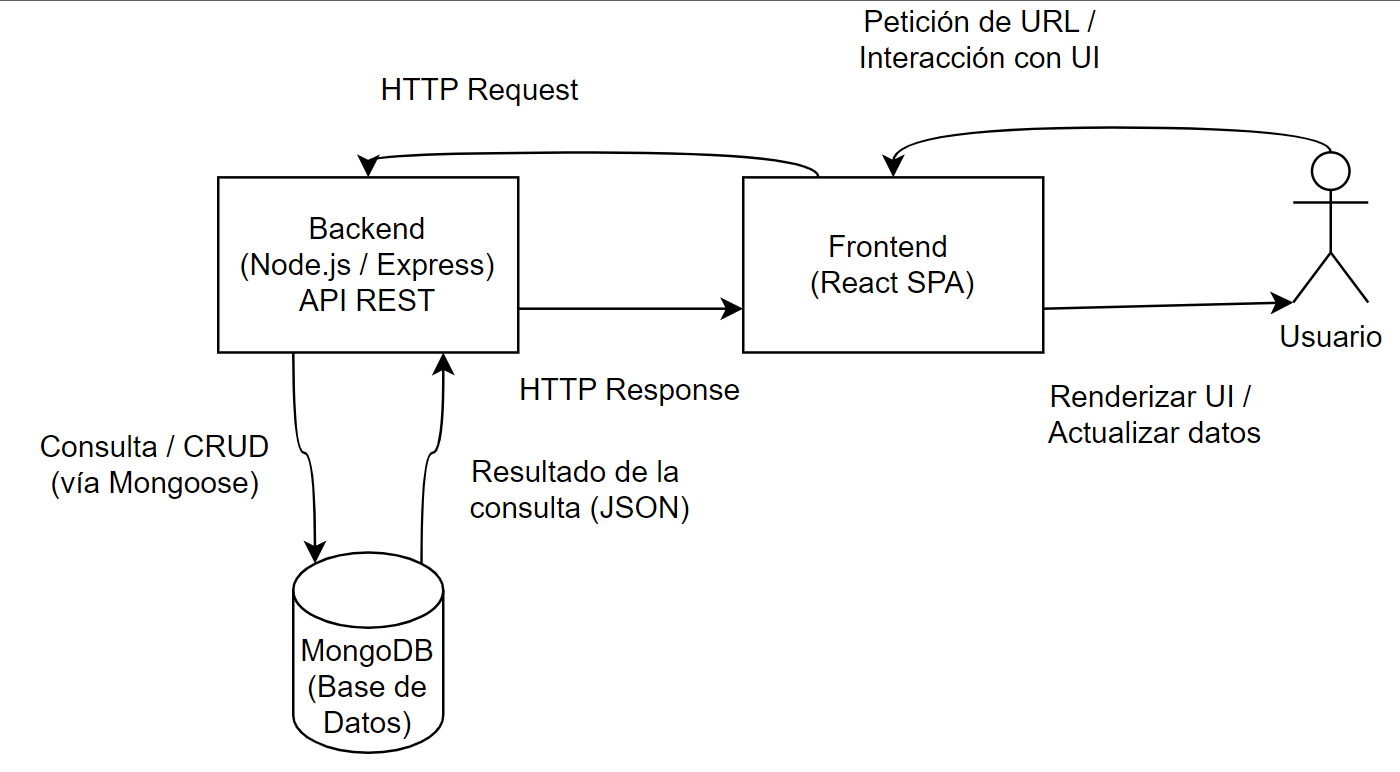
\includegraphics[clip=true,width=\textwidth]{img/arquitectura_logica_logart.png}\\

    \footnotesize (a)
  \end{minipage}
  \caption{Diagrama de Arquitectura Lógica de Alto Nivel de LogArt.}\label{fig:arquitecturaLogica}
  \end{figure}

\subsection{Arquitectura de Despliegue (Simplificada)}
\label{ssec:arquitecturaDespliegue}

La arquitectura lógica descrita anteriormente se implementa y despliega utilizando tecnología de contenerización, específicamente Docker y Docker Compose (ver Sección: \ref{sec:contenedores}). Este enfoque asegura la portabilidad, consistencia y facilidad de gestión del entorno de la aplicación, tanto para desarrollo como para una eventual puesta en producción.

Los componentes principales de la aplicación LogArt se empaquetan en contenedores Docker, la orquestación de estos contenedores se gestiona mediante Docker Compose.

La arquitectura de despliegue de LogArt se compone de los siguientes servicios principales definidos en el archivo \texttt{docker-compose.yml}

\begin{itemize}
    \item \textbf{Servicio \texttt{app} (Contenedor de la Aplicación LogArt):}
    \begin{itemize}
        \item Este contenedor ejecuta la aplicación backend Node.js/Express.js.
        \item También es responsable de servir los archivos estáticos del frontend React, que son compilados y copiados a una carpeta pública dentro de este contenedor durante el proceso de construcción de la imagen Docker (como se detalló en la Sección \ref{sec:contenedores} sobre el \texttt{Dockerfile} multi-etapa).
        \item Se expone un puerto para permitir el acceso a la aplicación desde el exterior del contenedor, utilizando HTTPS con certificados auto firmados para el entorno de desarrollo.
        \item La configuración específica del entorno (como credenciales de base de datos, secretos de API, etc) se gestiona mediante variables de entorno, cargadas a través de un archivo \texttt{.env}.
    \end{itemize}
    \item \textbf{Servicio \texttt{mongo} (Contenedor de la Base de Datos MongoDB):}
    \begin{itemize}
        \item Este contenedor ejecuta una instancia de la base de datos MongoDB.
        \item Utiliza una imagen oficial de MongoDB proveniente de DockerHub.
        \item La base de datos es accesible para el servicio \texttt{app} a través de una red interna definida por Docker Compose.
    \end{itemize}
\end{itemize}

Ambos servicios (\texttt{app} y \texttt{mongo}) están configurados con \textit{healthchecks} en el archivo \texttt{docker-compose.yml} para monitorizar su estado y gestionar dependencias de arranque, asegurando que, por ejemplo, la aplicación no intente conectarse a la base de datos antes de que esta esté completamente operativa.

\begin{figure}
   \centering

  \begin{minipage}{0.45\textwidth}
   \centering

     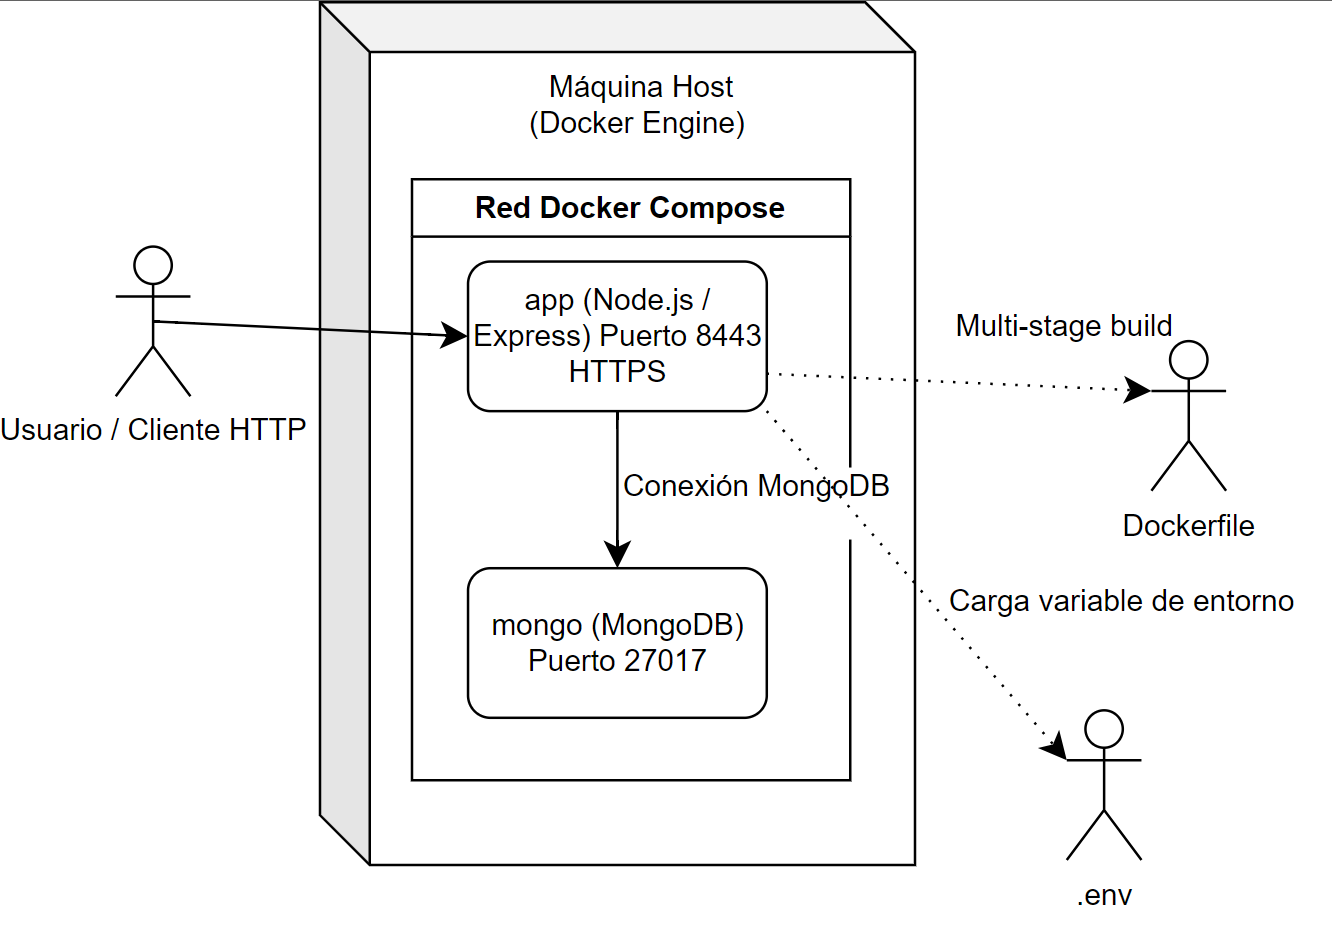
\includegraphics[clip=true,width=\textwidth]{img/arquitectura_despliegue_logart.png}\\

    \footnotesize (b)
  \end{minipage}
  \caption{Diagrama de Arquitectura de Despliegue Simplificado de LogArt.}\label{fig:arquitecturaDespliegue}
  \end{figure}

Esta arquitectura de despliegue basada en contenedores no solo facilita el entorno de desarrollo local, sino que también sienta las bases para despliegues más robustos en entornos de producción, ya que las mismas imágenes y configuraciones de Docker Compose pueden ser utilizadas en plataformas que soporten contenedores

\subsection{Diseño del Backend}
\label{ssec:disenoBackend}

El backend de LogArt, desarrollado con Node.js y el framework Express.js, ha sido estructurado siguiendo principios de modularidad y separación de responsabilidades para facilitar su desarrollo, mantenimiento y comprensión. A continuación, se describe su organización interna y el modelo de datos subyacente.

\subsubsection{Estructura de Directorios y Organización del Código}
\label{sssec:estructuraBackend}

El código fuente del backend de LogArt se organiza en una estructura de directorios que refleja una separación clara de las diferentes funcionalidades y capas de la aplicación. La estructura principal, ubicada dentro de la carpeta \texttt{LogArtApp/backend/}, es la siguiente (se omiten archivos de configuración o irrelevantes para centrarse en los directorios de lógica):

\begin{itemize}
    \item \textbf{\texttt{/config}:} Contiene archivos de configuración de la aplicación, como la configuración de la conexión a la base de datos, o la gestión de claves SSL para HTTPS.
    \item \textbf{\texttt{/controllers}:} Alberga los controladores de la aplicación. Cada controlador es responsable de manejar las peticiones HTTP entrantes para un recurso específico (ej. \texttt{userController.js}, \texttt{objectController.js}), validar los datos de entrada (requiriendo ayuda de middlewares y servicios de validación), invocar la lógica de negocio apropiada en los servicios, y formular la respuesta HTTP que se enviará al cliente.
    \item \textbf{\texttt{/middlewares}:} Contiene funciones middleware personalizadas que se utilizan en el flujo de procesamiento de peticiones Express.js. Por ejemplo, middleware para la autenticación y autorización de usuarios (verificando tokens JWT), manejo de subida de imágenes, o verificación de roles.
    \item \textbf{\texttt{/models}:} Define los esquemas y modelos de datos utilizando Mongoose. Cada archivo en este directorio (ej. \texttt{user.model.js}, \texttt{object.model.js}, \texttt{comment.model.js} describe la estructura de los documentos que se almacenarán en las colecciones de MongoDB, incluyendo los tipos de datos, validaciones, valores por defecto, índices y relaciones.
    \item \textbf{\texttt{/repositories}:} Esta capa, abstrae las interacciones directas con los modelos Mongoose, proporcionando una interfaz más genérica para el acceso a datos. Los servicios invocan a los repositorios en lugar de a los modelos directamente.
    \item \textbf{\texttt{/routes}:} Contiene los archivos que definen las rutas de la API RESTful. Cada archivo de ruta (ej. \texttt{/userRoutes.js}, \texttt{/objectRoutes.js}) agrupa los endpoints relacionados con un recurso específico y los asocia con las funciones controladoras correspondientes. Estos archivos son luego montados en la aplicación principal de Express.
    \item \textbf{\texttt{/Seeders}:} Incluye scripts para poblar la base de datos con datos iniciales de prueba (ej. usuarios administradores, disciplinas iniciales, datos de ejemplo para desarrollo). Estos scripts son útiles para configurar el entorno de desarrollo rápidamente.
    \item \textbf{\texttt{/services}:} Esta capa contiene la lógica de negocio principal de la aplicación. Los servicios son invocados por los controladores y son responsables de orquestar las operaciones, aplicar reglas de negocio, y interactuar con los repositorios para acceder y manipular los datos.
    \item \textbf{\texttt{/utils}:} Directorio para funciones de utilidad o helpers re utilizables, como el envío de correos, la validación de un id según MongoDB, o la función \texttt{notifyAdmins} con sockets.
    \item \textbf{\texttt{/\textunderscore \textunderscore test\textunderscore\textunderscore}:} Contiene los archivos de pruebas automatizadas para el backend, utilizando Jest y Supertest. \ref{sec:herramientasPruebas}
    \item \textbf{\texttt{/api-docs}:} Almacena la especificación OpenAPI (Swagger) generada para la documentación de la API.
\end{itemize}
Los archivos principales en la raíz del backend, como \texttt{app.js} (o \texttt{server.js}), se encargan de configurar e inicializar la aplicación Express, montar las rutas, aplicar middlewares globales e iniciar el servidor. Esta estructura modular facilita la navegación por el código, la adición de nuevas funcionalidades y el mantenimiento del sistema.

En la figura \ref{fig:diagramaClasesBackend} se muestra el diagrama de clases del backend.

\begin{figure}
   \centering

  \begin{minipage}{0.45\textwidth}
   \centering

     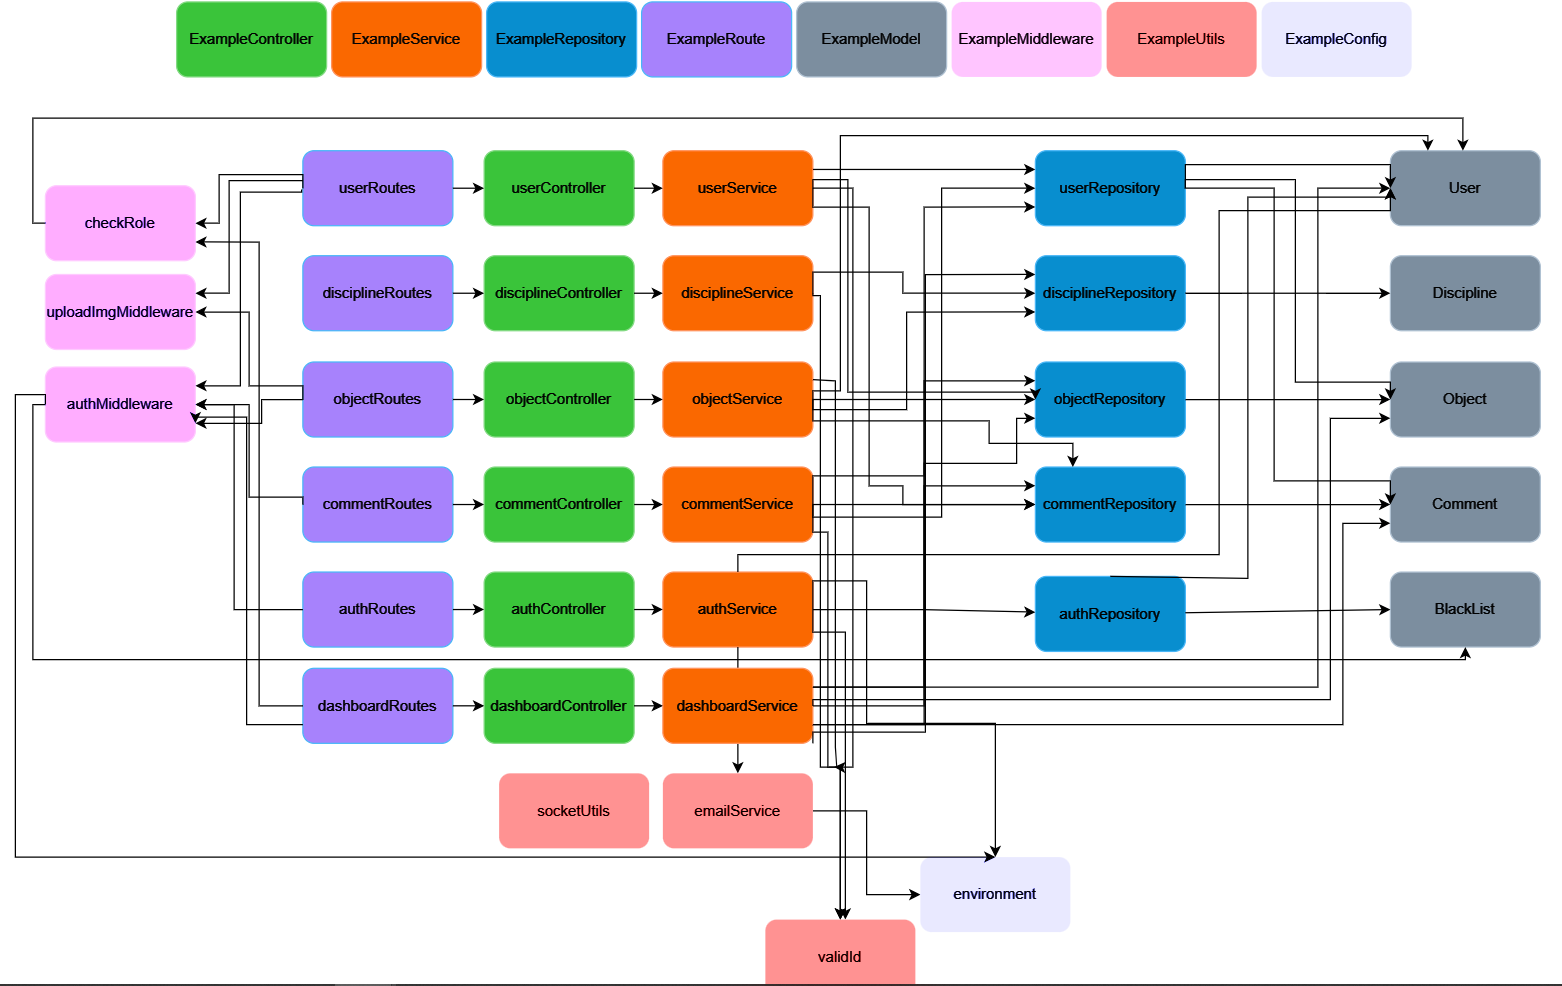
\includegraphics[clip=true,width=\textwidth]{img/diagrama_clases_backend_logart.png}\\

    \footnotesize (c)
  \end{minipage}
  \caption{Diagrama de Clases del Backend de la Aplicación.}\label{fig:diagramaClasesBackend}
  \end{figure}

\subsubsection{Modelo de Dominio y Diagrama de Clases del Backend}
\label{sssec:modeloDominioBackend}

El modelo de dominio del backend representa las entidades principales de LogArt y sus interrelaciones. Estas entidades se corresponden directamente con los modelos definidos mediante Mongoose y las colecciones en la base de datos MongoDB. Las entidades clave son:
\begin{itemize}
    \item \textbf{User (Usuario):} Representa a un usuario de la aplicación, con atributos como nombre de usuario, correo, contraseña (hasheada), nombre, apellidos, biografía, imagen de perfil, rol, entre otros.
    \item \textbf{Object (Objecto):} Representa una entrada de una obra creada por un usuario, asociada a una disciplina. Contiene atributos como título, descripción, imagen, fecha de creación, referencia al usuario propietario, y un indicador de si está compartido o no.
    \item \textbf{Comment (Comentario):} Representa una anotación o recuerdo detallado asociado a un \texttt{Object}. Contiene el texto del comentario, la fecha de creación, si ha sido por un admin o no, y el id del objeto al que pertenece.
    \item \textbf{Discipline (Disciplina):} Representa las categorías principales de la web, como ``Libros'', ``Canciones'' y ``Videojuegos''. Contiene simplemente el nombre de la entidad y la descripción.
    \item \textbf{BlackListedToken:} Representa un token en la lista negra, contiene el token y la fecha de caducidad, en la que será borrado automáticamente de la base de datos.
\end{itemize}

Las relaciones principales entre estas entidades son:
\begin{itemize}
    \item Un \texttt{User} puede crear muchos \texttt{Object's} (relación uno a muchos).
    \item Un \texttt{Object} pertenece a un solo \texttt{User} (propietario).
    \item Un \texttt{Object} puede tener muchos \texttt{Comment's} (relación uno a muchos).
    \item Un \texttt{Comment} pertenece a un solo \texttt{Object} y es creado por un \texttt{user}.
    \item Un \texttt{Object} está asociado a una \texttt{Discipline}.
    \item \texttt{BlackListToken} representa un token que ha sido invalidado por alguna razón, y por tanto, ha entrado en la lista negra.
\end{itemize}

En la figura \ref{fig:diagramaEntidadesBD} se  representa el diagrama de entidades de la base de datos, que ilustra estas entidades y sus relaciones. Mientras que en el \ref{fig:diagramaEntidadesBDSimple} se muestra a un nivel más alto de abstracción.

\begin{figure}
   \centering

  \begin{minipage}{0.45\textwidth}
   \centering

     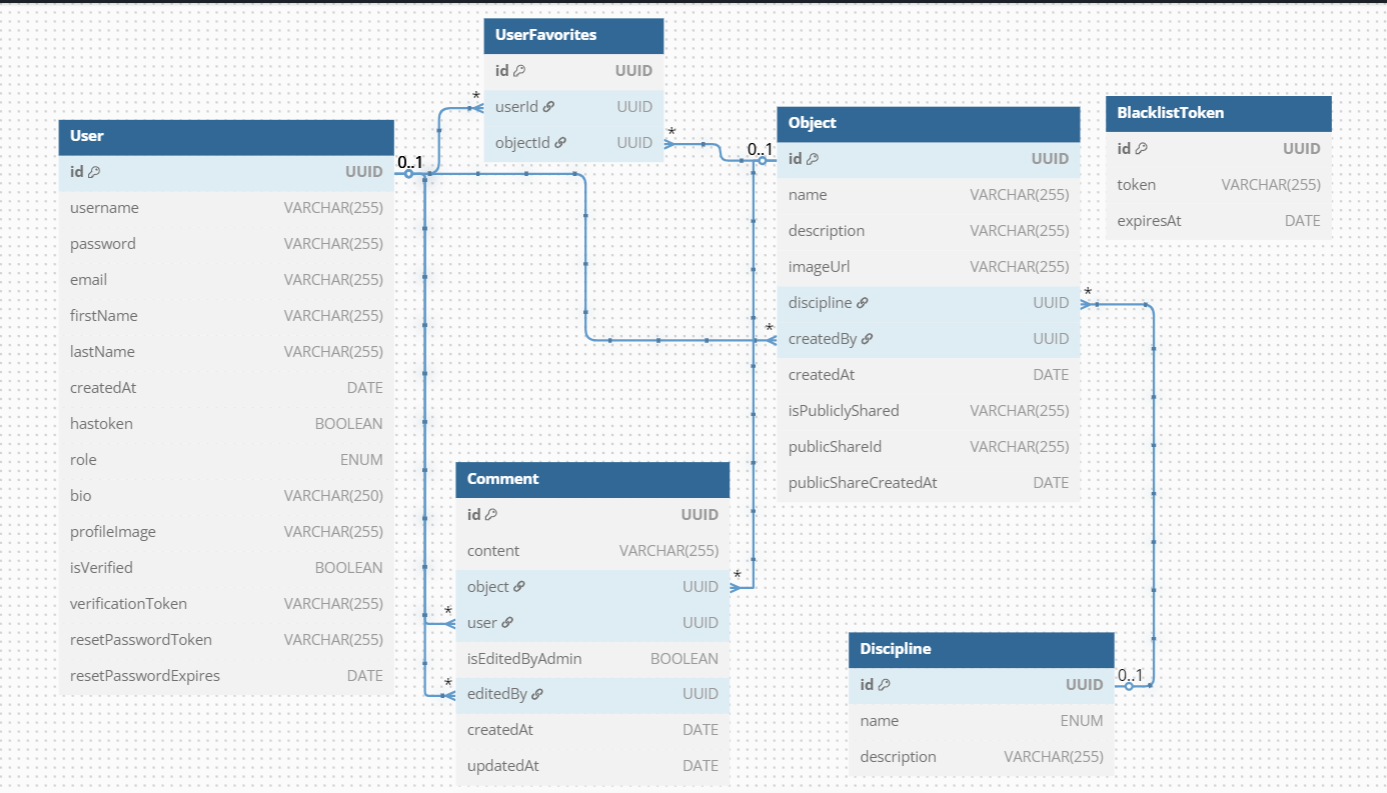
\includegraphics[clip=true,width=\textwidth]{img/diagrama_entidades_basedatos.png}\\

    \footnotesize (d)
  \end{minipage}
  \caption{Diagrama de Entidades de la Base de Datos.}\label{fig:diagramaEntidadesBD}
  \end{figure}

\begin{figure}
   \centering

  \begin{minipage}{0.45\textwidth}
   \centering

     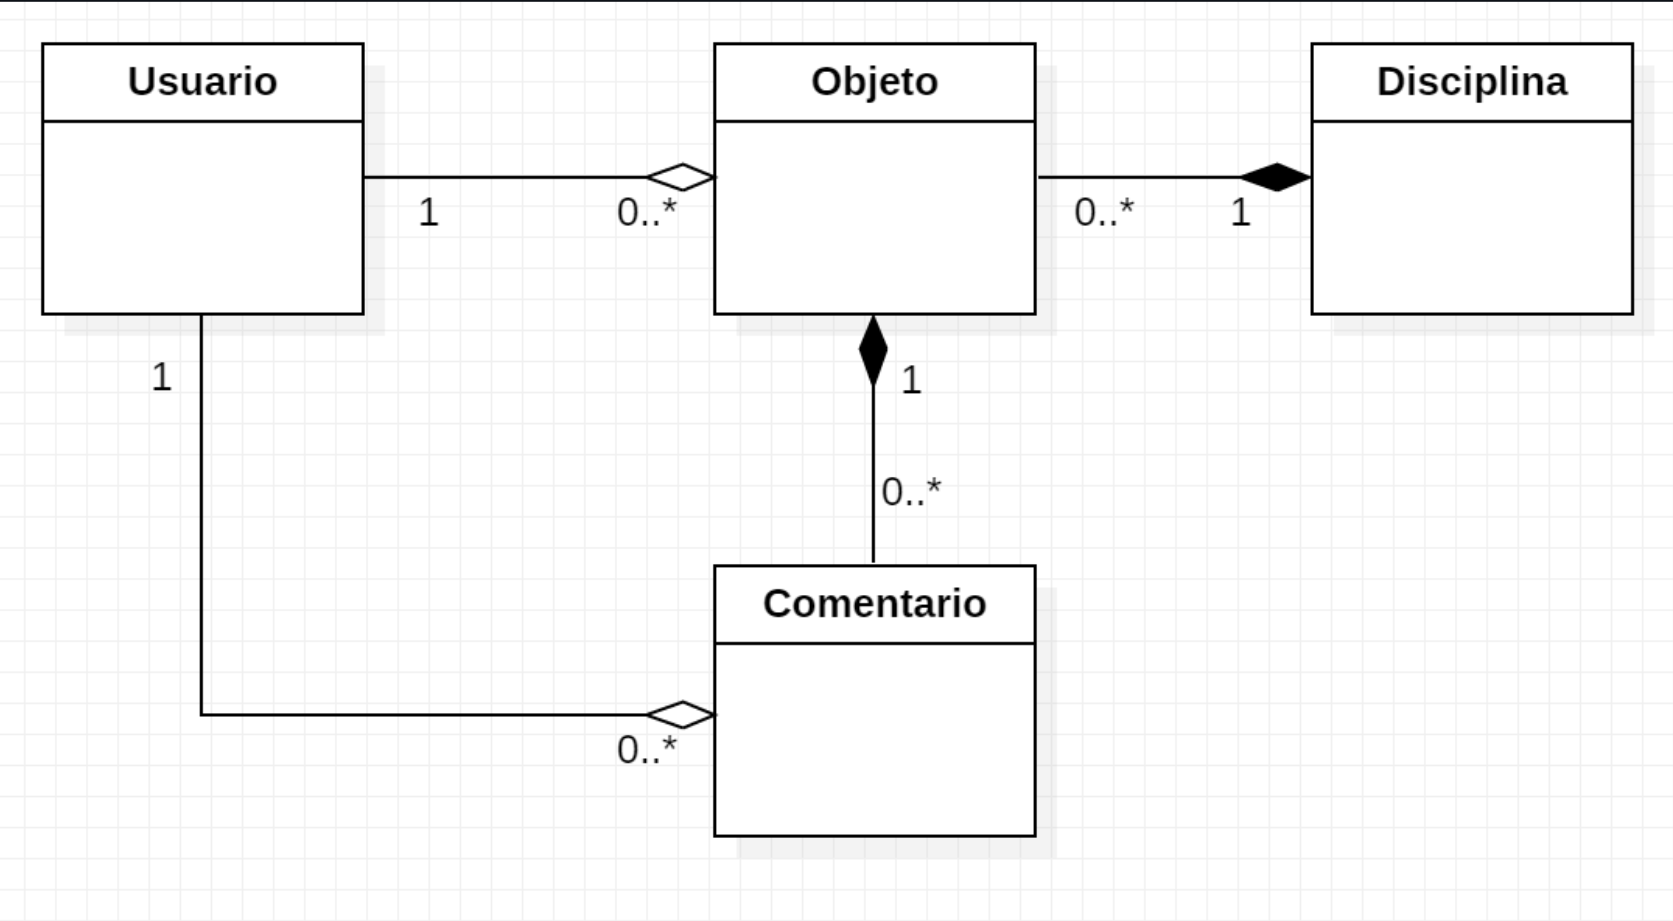
\includegraphics[clip=true,width=\textwidth]{img/diagrama_entidades_altonivel.png}\\

    \footnotesize (d.2)
  \end{minipage}
  \caption{Diagrama de Entidades de la Base de Datos, con mayor nivel de abstracción.}\label{fig:diagramaEntidadesBDSimple}
  \end{figure}

\subsection{Diseño del Frontend (Single Page Application)}
\label{ssec:disenoFrontend}

El frontend de LogArt se ha desarrollado como una Single Page Application (SPA) utilizando la biblioteca/framework React. Este enfoque permite una experiencia de usuario fluida y dinámica, donde las transiciones entre diferentes vistas y la actualización de contenido se realizan sin necesidad de recargar la página completa desde el servidor. La estructura y los componentes principales del frontend se describen a continuación.

\subsubsection{Estructura de Directorios y Organización de Componentes}
\label{sssec:estructuraFrontend}

El código fuente de LogArt, ubicado en la carpeta \texttt{/LogArt-frontend/}, se organiza para promover la modularidad y la reutilización de componentes. La estructura principal dentro del directorio \texttt{src/} es la siguiente:
\begin{itemize}
    \item \textbf{\texttt{/components}:} Este directorio contiene componentes de React reutilizables que se utilizan en diversas partes de la aplicación. Entre estos se incluyen componentes de UI genéricos (ej. botones, modales, tarjetas de objetos) o componentes más específicos que encapsulan la porción de la interfaz y su lógica. El objetivo es fomentar la composición y evitar la duplicación de código. Algunos ejemplos claves son:
    \begin{itemize}
        \item \texttt{CommentList.jsx}
        \item \texttt{DisciplineSelector.jsx}
        \item \texttt{Navbar.jsx}
        \item \texttt{ObjectCard.jsx}.
    \end{itemize} 
    \item \textbf{\texttt{/context}:} Aquí se definen los Contextos de React. La API de contexto de React se utiliza para gestionar el estado global o compartido entre componentes que no están directamente relacionados en el árbol de componentes.
    \begin{itemize}
        \item \texttt{AuthContext}: Gestiona el estado de autenticación del usuario (si está logueado, datos del usuario, token JWT) y proporciona funciones para iniciar y cerrar sesión.
        \item \texttt{ModalContext}: Controla la visibilidad y el contenido de los modales genéricos utilizados en la aplicación
        \item \texttt{SocketContext}: Administra la conexión y los eventos de WebSockets (Socket.IO) para funcionalidades en tiempo real, como las notificaciones del administrador.
    \end{itemize}
    \item \textbf{\texttt{/pages}:} Contiene los componentes de React que representan las diferentes ``páginas'' o vistas principales de la aplicación (ej. \texttt{Hero.jsx}, \texttt{ObjectDetail.jsx}, \texttt{Profile.jsx}). Estos componentes se componen de varios componentes más pequeños del directorio \texttt{/components} y gestionan la lógica específica de cada vista.
    \item \textbf{\texttt{/utilities}:} Directorio para funciones o archivos de utilidad, como \texttt{api.js} que centraliza las llamadas a la API con Axios, o \texttt{faqs.jsx}, que contiene las preguntas y respuestas que se mostrarán en la página inicial.
    \item \textbf{\texttt{App.jsx}:} Es el componente raíz de la aplicación React. Se encarga de configurar el enrutador (React Router DOM) y de renderizar los componentes de página según la ruta actual.
    \item \textbf{\texttt{main.jsx}:} Es el punto de entrada de la aplicación React, donde se renderiza el componente \texttt{App.jsx}.
    \item \textbf{\texttt{/ui-test/tests}:} Directorio que alberga las pruebas End-to-End implementadas con Playwright para validar la interfaz de usuario y los flujos de interacción.
\end{itemize}

Esta organización busca mantener el código ordenado, facilitando la localización de componentes y la facilidad de desarrollo.

En la Figura \ref{fig:diagramaComponentesFrontend} se presenta un diagrama que ilustra la relación entre: componentes, páginas, contexto y utilidad, mostrando como se componen para formar las diferentes vistas que el usuario experimenta. El diagrama se enfoca en la estructura y las relaciones entre componentes, más que en el flujo de datos detallado, para ofrecer una visión general de la arquitectura de la SPA.

\begin{figure}
   \centering

  \begin{minipage}{0.45\textwidth}
   \centering

     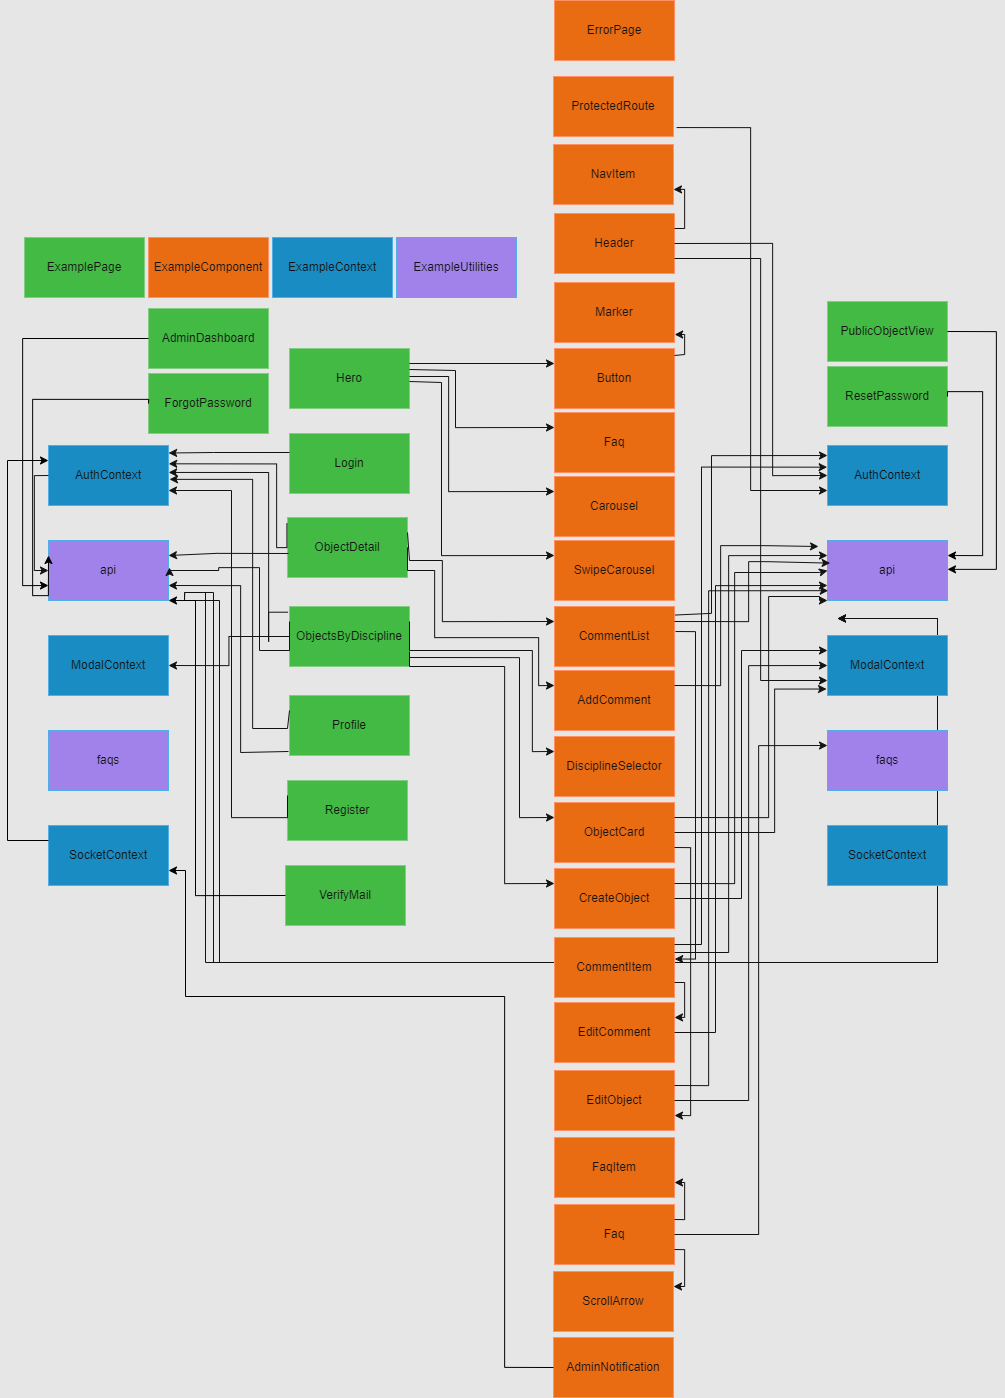
\includegraphics[clip=true,width=\textwidth]{img/diagrama_componentes_frontend_logart.png}\\

    \footnotesize (e)
  \end{minipage}
  \caption{Diagrama de Componentes Frontend de la aplicación.}\label{fig:diagramaComponentesFrontend}
  \end{figure}

\section{Diseño e Implementación}
\label{sec:disenoImplementacion}

Tras la descripción de la arquitectura general de LogArt en la sección anterior, este apartado se adentra en los detalles concretos del diseño interno y la implementación de sus componentes y funcionalidades clave. El objetivo es ofrecer una visión más profunda de cómo se han traducido los requisitos y las decisiones arquitectónicas en código funcional, destacando las soluciones técnicas adoptadas, y algunos de los aspectos más relevantes del proceso de desarrollo.

Se explorarán tanto el diseño del backend, centrándose en la estructura de su API RESTful y la integración con la base de datos, como el diseño frontend, detallando la gestión del estado y la composición de la interfaz de usuario en React. Además, se abordarán aspectos específicos de la implementación, como la resolución de desafíos técnicos particulares o la descripción de una funcionalidad destacada del sistema. 

Este análisis detallado busca no solo documentar la aplicación construida, sino también justificar las decisiones e implementación tomadas, proporcionando al lector una comprensión clara de la ingeniería detrás de LogArt.

\subsection{Diseño e Implementación del Backend}
\label{ssec:disenoImplBackend}

El backend de LogArt, construido sobre Node.js y Express.js, es el responsable de la lógica de negocio, la gestión de datos y la exposición de una API RESTful. Su diseño se ha centrado en la modularidad, la separación de responsabilidades y la seguridad.

\subsubsection{API RESTful: Diseño y Flujo de Peticiones}
\label{sssec:apiRestfulDiseno}

La comunicación entre el frontend y el backend se realiza a través de una API RESTful. Se han seguido los principios estándar de diseño REST, como el uso de métodos HTTP semánticos (GET, POST, PUT, DELETE), la representación de recursos a través de URLs claras y el uso de códigos de estado HTTP para indicar el resultado de las operaciones. Todas las respuestas de la API se devuelven en formato JSON.

La estructura de las rutas de la API, definidas en el directorio \texttt{/routes} ( por ejemplo \texttt{objectRoutes.js}, sigue un patrón basado en recursos. Por ejemplo, todas las operaciones relacionadas con los ``objetos'' se agrupan bajo el prefijo \texttt{/api/v1/objects}. El archivo \texttt{app.js} centraliza la configuración de la aplicación Express, incluyendo el montaje de estas rutas y la aplicación de middlewares globales como \texttt{cors} (para la gestión de Intercambio de Recursos de Origen Cruzado) y \texttt{express.json()} (para el parseo de cuerpos de petición JSON).

El flujo típico de una petición a un endpoint protegido es el siguiente:
\begin{enumerate}
    \item El cliente (frontend), a través de alguna acción en la interfaz, realiza una petición HTTP a un endpoint de la API, incluyendo un JSON Web Token (JWT) en la cabecera \texttt{Authorization} (ej. \texttt{Bearer token}).
    \item La petición llega a la aplicación Express.js
    \item El middleware de autenticación (\texttt{verifyToken} en \texttt{authMiddleware.js})  intercepta la petición. Este middleware:
    \begin{itemize}
        \item Verifica la presencia y validez del token JWT.
        \item Comprueba si el token está en una lista negra (modelo \texttt{BlaclistedToken}) para tokens revocados (ej. tras un cierre de sesión).
        \item Si el token es válido y no está en la lista negra, decodifica el payload del usuario (que incluye \texttt{userId} y \texttt{role}) y los adjunta al objeto \texttt{req} (ej. \texttt{req.user}).
        \item Si el token es inválido o no se proporciona, se devuelve una respuesta de error (401 no Autorizado o 403 Prohibido).
    \end{itemize}
    \item Si la autenticación es exitosa, la petición pasa al siguiente punto de la validación.
    \item El controlador extrae los datos necesarios de la petición (\texttt{req.params}, \texttt{req.body}, \texttt{req.query} y \texttt{req.file} para subida de archivos con \texttt{multer}, como se puede ver en \texttt{objectRoutes.js} para la creación y actualización de objetos).
    \item El controlador invoca la función apropiada en el módulo de servicio correspondiente (ej. \texttt{objectService.js}), pasándole los datos validados y el \texttt{userId} del usuario autenticado.
    \item El servicio aplica la lógica de negocio, interactuando con los repositorios (ej. \texttt{objectRepository.js}) que a su vez operan sobre los modelos Mongoose (ej. \texttt{object.model.js}) para realizar las operaciones CRUD en la base de datos MongoDB.
    \item El servicio devuelve el resultado (o un error) al controlador.
    \item El controlador construye la respuesta HTTP (Código de estado, cabeceras como \texttt{Location} para creaciones exitosas, y cuerpo JSON) y la envía de vuelta al cliente.
\end{enumerate}

Un ejemplo de este flujo se puede observar en la creación de un objeto (controlador \texttt{createObject} en \texttt{objectController.js}): 
\begin{itemize}
    \item La ruta \texttt{POST /api/v1/objects} está protegida por \texttt{verifyToken} y utiliza el middleware \texttt{uploadObject.single(``imageUrl'')} para manejar la subida de la imagen.
    \item El controlador luego llama a \texttt{objectService.createObject}, que valida los datos, interactúa con \texttt{disciplineRepository} y \texttt{objectRepository}, y finalmente devuelve el objeto creado o un error.
    \item El controlador entonces responde al cliente con un estado 201 y la ubicación del nuevo recurso.
     
\end{itemize}   
La documentación de la API, generada con Swagger a partir de anotaciones JSDoc en los controladores, detalla todos los endpoints disponibles, sus parámetros y esquemas de respuesta.

\subsubsection{Interacción con la Base de Datos y Lógica de Negocio}
\label{sssec:backendDbLogica}

La persistencia de datos se gestiona a través de MongoDB, con una capa de abstracción proporcionada por Mongoose. Los modelos (ej. \texttt{object.model.js}) definen la estructura de los datos, incluyendo tipos, campos requeridos, valores por defecto, relaciones mediante \texttt{Schema.Types.ObjectId} y la propiedad \texttt{ref}.

Los \textbf{repositorios} (ej. \texttt{objectRepository.js}) encapsulan las consultas directas a la base de datos utilizando los modelos Mongoose. Proporcionan métodos específicos para las operaciones CRUD y consultas más complejas (ej. \texttt{findObjects} con filtros, paginación y populación de campos referenciados; \texttt{findByPublicShareId}). Esta capa de repositorio ayuda a desacoplar la lógica de negocio de los detalles de implementación de Mongoose.

Los \textbf{servicios} (ej. \texttt{objectService.js} contienen la lógica de negocio principal. Por ejemplo, el servicio \texttt{objectService}:
\begin{itemize}
    \item Valida la existencia de disciplinas antes de crear o actualizar un objeto.
    \item Verifica los permisos del usuario para actualizar o eliminar un objeto, permitiendo estas acciones solo al propietario o a un administrador.
    \item Gestiona la eliminación de imagen asociadas cuando un objeto se actualiza o elimina (evitando dejar archivos huérfanos, con la excepción de las imágenes por defecto).
    \item Maneja la lógica para compartir públicamente un objeto, generando un id único (\texttt{publicShareId}) y gestionando su estado \texttt{isPubliclyShared}.
    \item En la función \texttt{togglePublicShare}, interactúa con \texttt{socketUtils} para notificar a los administradores cuando un objeto se comparte, demostrando la integración con WebSockets.
\end{itemize}

En resumen, el diseño del backend de LogArt se ha organizado de forma modular para garantizar la separación de responsabilidades entre rutas, controladores, servicios y repositorios. Gracias al uso de middleware para autenticación, la lógica de validación y la de gestión de errores, así como a la abstracción de la persistencia mediante Mongoose, conseguimos un API RESTful robusto, seguro y fácil de mantener. Además, la integración con Swagger facilita la generación ``Automática'' de la documentación.

A continuación, en la Sección \ref{ssec:disenoImplFrontend}, abordaremos el diseño e implementación del frontend en React, donde veremos cómo esta capa consume la API, maneja el estado de la aplicación y construye la interfaz de usuario en LogArt.

\subsection{Diseño e Implementación del Frontend (React)}
\label{ssec:disenoImplFrontend}

El frontend de LogArt, desarrollado como un Single Page Application (SPA) con React, es el punto de interacción directo con el usuario. Su diseño se ha enfocado en la creación de una interfaz intuitiva, responsiva y modular, utilizando componentes reutilizables y una gestión de estado eficiente.

\subsubsection{Gestión de Estado con Context API}
\label{sssec:frontendEstadoContext}

Para gestionar el estado global o compartido a través de diferentes componentes de la aplicación se ha utilizado la API de contexto de React. Los principales contextos implementados son:

\begin{itemize}
    \item \textbf{\texttt{AuthContext.jsx}:} Este contexto es fundamental para la gestión de la autenticación del usuario.
    \begin{itemize}
        \item Mantiene el estado del usuario actual (\texttt{user}), un booleano \texttt{isAuthenticated} que indica si el usuario ha iniciado sesión, y un estado de carga \texttt{loading} para gestionar la verificación inicial del token.
        \item Almacena el token JWT el \texttt{localStorage} tras un inicio de sesión exitoso y lo configura en las cabeceras por defecto de Axios (ver \texttt{utilities/api.jsx}).
        \item Intenta cargar el perfil del usuario al iniciarse la aplicación si existe un token en \texttt{localStorage}, manteniendo así la sesión del usuario entre recargas.
        \item Proporciona funciones para \texttt{login}, \texttt{register}, \texttt{logout}, que encapsulan las llamadas a la API del backend y actualizan el estado de autenticación en consecuencia. La función \texttt{logout} también se encarga de eliminar el token de \texttt{localStorage} y de la lista negra del backend.
    \end{itemize}
    \item \textbf{\texttt{ModalContext.jsx}:} Proporciona una forma centralizada de gestionar la apertura y cierre de componentes modales genéricos en toda la aplicación.
    \begin{itemize}
        \item Mantiene el estado del modal actualmente visible (\texttt{currentModal}) y sus propiedades (\texttt{modalProps}).
        \item Ofrece funciones \texttt{openModal} (que recibe el componente modal a renderizar y sus props) y \texttt{closeModal}.
        \item Incluye un efecto (\texttt{useEffect}) para deshabilitar el scroll del cuerpo de la página cuando un modal está activo, mejorando la experiencia de usuario. El componente modal se renderiza directamente desde el proveedor del contexto.
    \end{itemize}
    \item \textbf{\texttt{SocketContext.jsx}:} Gestiona la conexión y los eventos de WebSockets para funcionalidades en tiempo real. Este contexto encapsula la lógica de conexión al servidor de sockets y la suscripción/emisión de eventos.
\end{itemize}

Además del estado global gestionado por Context, los componentes individuales utilizan el estado local (\texttt{useState}, \texttt{useEffect}) para manejar su propia lógica de UI y datos temporales.

\subsubsection{Flujo de Datos y Comunicación con la API}
\label{sssec:frontendFlujoDatosApi}

La interacción con la API RESTful del backend se centraliza principalmente a través de una instancia de Axios configurada en \texttt{utilities/api.jsx}. Esta instancia define la \texttt{baseURL} del servidor backend (\texttt{https://localhost:8443}) y utiliza interceptores de petición para adjuntar automáticamente el token JWT (obtenido de \texttt{localStorage} a través del \texttt{AuthContext}) a la cabecera \texttt{Authorization} de cada solicitud, simplificando las llamadas a endpoints protegidos.

Los componentes de página (ubicados en \texttt{/pages}), como \texttt{ObjectsByDiscipline.jsx}, son generalmente responsables de:
\begin{itemize}
    \item Obtener los datos necesarios para su vista al montarse (utilizando \texttt{useEffect} y funciones asíncronas que llaman al servicio \texttt{api}).
    \item Manejar la lógica de paginación, búsqueda (con debounce como se puede ve en \texttt{ObjectsByDiscipline.jsx} para optimizar las peticiones mientras el usuario escribe) y filtrado (ej. ``mostrar solo favoritos'').
    \item Pasar los datos y funciones de callback necesarias a los componentes de prestación hijos.
    \item Actualizar su estado local (y, por ende, la UI) en respuesta a las acciones del usuario o a los datos recibidos de la API.
\end{itemize}
El componente \texttt{App.jsx} actúa como el orquestador principal del frontend, configurando el enrutador \texttt{react-router-dom} para mapear las URLs a los componentes de página correspondientes. Utiliza el componente \texttt{ProtectedRoute} para restringir el acceso a ciertas rutas basándose en el estado de autenticación del usuario y, opcionalmente, en su rol (ej. para el \texttt{/admin/dashboard}).

\subsubsection{Componentes Reutilizables Clave}
\label{sssec:frontendComponentesReutilizables}

La modularidad del frontend se logra mediante el uso extensivo de componentes reutilizables, algunos ejemplos destacados son:
\begin{itemize}
    \item \textbf{\texttt{Header.jsx}: } Componente estructural presente en la mayoría de las vistas, proporcionando navegación principal y enlaces comunes.
    \item \textbf{\texttt{DisciplineSelector.jsx}:} Un componente de UI que permite al usuario seleccionar una disciplina de una lista desplegable. Gestiona su propio estado de apertura y maneja la selección del usuario, notificando al componente padre del cambio.
    \item \textbf{\texttt{ObjectCard.jsx}:} Representa la vista en miniatura de un objeto en la galería. Muestra información clave del objeto (imagen, nombre, descripción breve, creador) y proporciona acciones como editar, eliminar (si el usuario es el propietario) y marcar/desmarcar como favorito. Este componente encapsula la lógica para estas acciones, incluyendo las llamadas a la API y la actualización del estado local o global (a través de callbacks o contexto).
    \item \textbf{\texttt{CreateObject.jsx} y \texttt{(EditObject.jsx}):} Componentes modales (gestionados por \texttt{ModalContext}) que presentan formularios para la creación y edición de objetos. Manejan el estado del formulario, la validación de entrada, la subida de imágenes (\texttt{multipart/form-data}) y la comunicación con la API para persistir los cambios.
    \item \textbf{\texttt{ProtectedRoute.jsx}:} Un componente de orden superior que envuelve rutas para restringir el acceso solo a usuarios autenticados y, opcionalmente, a roles específicos (ej. \texttt{admin}). Redirige a la página de inicio de sesión si no se cumplen las condiciones.
\end{itemize}

Estos componentes, entre muchos otros, permiten construir interfaces complejas de forma eficiente y mantener una base de código organizada.

\subsection{Foco en una Parte del Desarrollo: El Panel de Administración}
\label{ssec:focoAdminDashboard}

Una de las funcionalidades avanzadas y más complejas implementadas en LogArt es el Panel de Administración o Admin Dashboard. Esta sección está diseñada para proveer al rol de Administrador una visión general del estado de la plataforma, estadísticas detalladas sobre usuarios y contenido, y herramientas para la moderación. A continuación, se detalla su diseño e implementación tanto en el backend como en el frontend.
\paragraph{Requisitos Específicos del Admin Dashboard:}
El dashboard debía cumplir con los siguientes requisitos funcionales principales (derivados de RF6 en la Sección \ref{rf:adminFuncionalidades}):
\begin{itemize}
    \item Presentar un resumen general (overview) con métricas clave (total de usuarios, objetos, comentarios).
    \item Ofrecer estadísticas detalladas sobre los usuarios (distribución por rol, usuarios más activos).
    \item Proporcionar un análisis del contenido (distribución de objetos por disciplina, objetos más comentados).
    \item Mostrar la actividad de creación de contenido a lo largo del tiempo (semanal, mensual, trimestral).
    \item Analizar el crecimiento de usuarios, objetos y comentarios comparando periodos.
    \item Permitir la visualización y moderación (eliminación) de todos los objetos y usuarios de la plataforma.
    \item Ser accesible únicamente por usuarios con el rol de ``admin''.
\end{itemize}

\paragraph{Diseño e Implementación en el Backend:}El backend expone una serie de endpoints específicos bajo la ruta \texttt{/api/v1/dashboard/}, todos protegidos para ser accesibles únicamente por administradores mediante el middleware \texttt{authMiddleware.js}
\begin{itemize}
    \item \textbf{Rutas y Controladores:} El archivo \texttt{dashboardRoutes.js} define las rutas para cada sección del dashboard (ej. \texttt{/overview} , \texttt{/activity, etc}). Cada ruta está asociada a una función en \texttt{dashboardController.js}, que actúa como intermediario, recibiendo la petición y llamando al servicio correspondiente.
    \item \textbf{Servicio del Dashboard (\texttt{dashboardService.js}):} Este servicio es el corazón de la lógica del dashboard en el backend. Contiene funciones que realizan agregaciones complejas y consultas a la base de datos MongoDB utilizando los modelos Mongoose (a través de los repositorios) para recopilar y procesar los datos necesario para cada estadística. Destacan las siguientes funcionalidades:
    \begin{itemize}
        \item \textbf{Agregaciones con MongoDB Aggregate Framework:} Para muchas estadísticas, como \texttt{objectsByDiscipline}, \texttt{usersByRole}, \texttt{usersByObjectCount}, y \texttt{mostCommentedObjects}, se utiliza el potente \textit{Aggregation Framework} de MongoDB. Por ejemplo, para \texttt{objectsByDiscipline}, se realiza un \texttt{\$lookup} para unir con la colección de disciplinas y luego un \texttt{\$group} para contar objetos por nombre de disciplina.
        \item \textbf{Cálculo de Crecimiento:} La función \texttt{getGrowthAnalysis} calcula el porcentaje de crecimiento para usuarios, objetos y comentarios comparando el periodo actual (semanal, mensual, trimestral) con el periodo inmediatamente anterior. Utiliza una función auxiliar \texttt{calculateGrowthPercentage}.
        \item \textbf{Análisis de Actividad Temporal:} La función \texttt{getActivityStats} agrupa la creación de objetos por periodos (diario, semanal, mensual) utilizando \texttt{\$dateToString} en el pipeline de agregación para formatear las fechas de creación.
        \item \textbf{Paginación y Filtrado para Moderación:} La función \texttt{getAllObjects} permite al administrador obtener una lista paginada de todos los objetos, con opciones para filtrar por disciplina y término de búsqueda, facilitando la moderación.
    \end{itemize}
    El servicio se encarga de interactuar con las diferentes capas de repositorio para obtener los datos crudos y luego los transforma y agrega para presentar las estadísticas de forma útil.
\end{itemize}

A continuación, un fragmento simplificado de \texttt{dashboardService.js} que ilustra el uso del Aggregation Framework para obtener los objetos por disciplina:

\begin{lstlisting}[style=miJavaScript, caption=Ejemplo de agregación en \texttt{dashboardService.js} para \texttt{objectsByDiscipline}, label=lts:dashboardServiceAggregation]
const objectsByDiscipline = await Object.aggregate([
  {
    $lookup: { // Unir con la coleccion 'disciplines'
      from: "disciplines",
      localField: "discipline", // Campo en la coleccion 'objects'
      foreignField: "_id",      // Campo en la coleccion 'disciplines'
      as: "disciplineInfo",   // Nombre del nuevo array campo
    },
  },
  { $unwind: "$disciplineInfo" }, // Deconstruir el array disciplineInfo
  {
    $group: { // Agrupar por nombre de disciplina
      _id: "$disciplineInfo.name",
      count: { $sum: 1 }, // Contar objetos en cada grupo
    },
  },
  { // Proyectar el resultado final
    $project: { _id: 0, discipline: "$_id", count: 1 },
  },
]);
\end{lstlisting}
Este tipo de consultas permite procesar grandes volúmenes de datos directamente en la base de datos, optimizando el rendimiento.


\paragraph{Diseño e Implementación en el Frontend (\textbf{AdminDashboard.jsx} y componentes hijos):}

El frontend del Admin Dashboard, implementado como un componente React Principal (\texttt{AdminDashboard.jsx}), se encarga de presentar la información de forma organizada y permitir la interacción del administrador.
\begin{itemize}
    \item \textbf{Estructura de Pestañas (Tabs):} La interfaz del dashboard se organiza en varías pestañas (Resumen, Usuarios, Contenido, Actividad, Crecimiento, Objetos), cada una correspondiente a una sección de datos. El \texttt{AdminDashboard.jsx} se gestiona el estado de la pestaña activa (\texttt{activeTab}) y renderiza el contenido correspondiente. La navegación entre pestañas se actualiza utilizando \texttt{useEffect} para observar cambios en \texttt{location.pathname}.
    \item \textbf{Obtención de Datos:} Al cambiar de pestaña o de periodo (para Actividad y Crecimiento), se realiza una petición a la API del backend (usando la instancia de Axios configurada) para obtener los datos específicos de esa sección. Se manejan estados de carga (\texttt{loading}) y error (\texttt{error}) para informar al usuario.
    \item \textbf{Componentización de Vistas:} Cada pestaña tiene componentes dedicados para renderizar sus datos (\texttt{OverviewTab}, \texttt{UsersTab}, \texttt{GrowthTab} entre otros). Estos componentes reciben los datos obtenidos del backend como props y los presentan utilizando elementos de UI como tarjetas de estadísticas (\texttt{StatCard}), tablas y gráficos.
    \item \textbf{Interactividad y Moderación:} 
    \begin{itemize}
        \item En la pestaña ``Usuarios'' (\texttt{UsersTab}), se muestra una lista paginada de usuarios y se ofrece la opción de eliminar usuarios (excepto otros administradores). La eliminación de un usuario desencadena una petición DELETE a la API (junto con sus recursos asociados) y actualiza la UI localmente y las estadísticas del dashboard.
        \item En la pestaña ``Objetos'' (\texttt{ObjectsTab}), se implementa una interfaz para buscar para buscar, filtrar por disciplina y ver una lista paginada de todos los objetos. Se permite al administrador navegar a la vista detallada del objeto o eliminarlo directamente.
    \end{itemize}
    \item \textbf{Visualización de Datos:} Se utilizan componentes como \texttt{StatCard} y \texttt{GrowthCard} para presentar métricas de forma clara. La pestaña \texttt{ActivityTab} intenta representar un gráfico de barras para la actividad de creación de objetos, calculando la altura de las barras dinámicamente.
\end{itemize}
El diseño busca ofrecer una interfaz clara y funcional que permita al administrador acceder rápidamente a la información relevante y realizar acciones de moderación de forma eficiente.

Este desarrollo integrado entre el backend (con sus servicios de agregación de datos) y el frontend (con su estructura de componentes y gestión de estado) permite ofrecer una herramienta de administración potente y útil para la supervisión de LogArt.

\section{Pruebas}
\label{sec:pruebasCap4}

La validación del correcto funcionamiento y la robustez de LogArt ha sido un componente integral del proceso de desarrollo. Se implementó una estrategia de pruebas automáticas multinivel para asegurar la calidad del código y facilitar la detección temprana de regresiones. Estas pruebas, ejecutadas regularmente y como parte del pipeline de Integración Continua, se complementaron con pruebas manuales exploratorias.

\begin{itemize}
    \item \textbf{Pruebas del Backend (API RESTful):}
    \begin{itemize}
        \item Se desarrollaron pruebas de integración y unitarias para el backend utilizando el framework \textbf{Jest} y la librería \textbf{Supertest}. Estas pruebas se enfocaron en validar la lógica de los controladores, los servicios y la interacción con la base de datos (a través de los repositorios y modelos Mongoose)
        \item Se crearon suites de pruebas específicas para cada conjunto de funcionalidades principales, como se evidencia en los archivos de prueba:
        \begin{itemize}
            \item \texttt{auth.test.js}: Cubre los flujos de registro, inicio de sesión y cierre de sesión.
            \item \texttt{user.test.js}: Valida la gestión de perfiles de usuario y funcionalidades relacionadas con favoritos.
            \item \texttt{object.test.js}: Prueba la creación, actualización, eliminación y obtención de objetos, incluyendo las funcionalidades de compartir y marcar como favorito.
            \item \texttt{comment.test.js}: Asegura el correcto funcionamiento de la creación, edición, eliminación y obtención de comentarios.
            \item \texttt{discipline.test.js}: Valida la obtención de las disciplinas.
            \item \texttt{dashboard.test.js}: Verifica los diferentes endpoints del panel de administración asegurando la correcta agregación y presentación de las estadísticas.
        \end{itemize}
        \item Estas pruebas simulan peticiones HTTP a los endpoints de la API, verificando los códigos de estado, la estructura y contenido de las respuestas JSON, y los efectos secundarios en la base de datos
    \end{itemize}
    \vspace{0.3cm}
    \item \textbf{Pruebas End-To-End (E2E) del Frontend:}
    \begin{itemize}
        \item Para el frontend React, se implementaron pruebas E2E con \textbf{Playwright}. Estas pruebas automatizan la interacción con la interfaz de usuario en un navegador (Chromium), validando flujos completos desde la perspectiva del usuario, como el registro, inicio de sesión, creación de objetos y comentarios, la navegación, y la edición de perfil.
    \end{itemize}
    \vspace{0.3cm}
    \item \textbf{Integración con el Pipeline de CI/CD:}
    \begin{itemize}
        \item Como se describió en la Sección \ref{sec:cicd}, tanto las pruebas del backend como las pruebas E2E del frontend se integran en el workflow de Integración Continua de GitHub Actions. Se ejecutan automáticamente ante cada \textit{Pull Request} a la rama \texttt{main}, proporcionando una capa de seguridad esencial antes de integrar nuevos cambios.
    \end{itemize}
\end{itemize}

\paragraph{Cobertura de Código del Backend:}
Las pruebas automatizadas del backend, gestionadas con Jest, proporcionan una medida cuantitativa de la exhaustividad de las pruebas. Según el informe de cobertura generado (ver Figura \ref{fig:coberturaBackend}), se alcanzó una cobertura global del:
\begin{itemize}
    \item \textbf{69.76\%} en Statements (1057/1515)
    \item \textbf{59.91\%} en Branches (293/489)
    \item \textbf{64.37\%} en Functions (103/160)
    \item \textbf{69.89\%} en Lines (1054/1508)
\end{itemize}
Si bien hay áreas con alta cobertura, como los modelos y rutas (ambos al 100\% en Statements y Lines), y los repositorios (89.1\%), otras áreas como los Seeders (26.97\%) y algunos servicio o controladores específicos presentan una cobertura menor, indicando puntos donde se podrían añadir pruebas adicionales para incrementar la robustez. No obstante, se priorizó la cobertura de las funcionalidades críticas, la lógica de negocio principal, y las funciones más usadas de la aplicación, mientras que no se dio tanta importancia a testear cosas como los Seeders de la base de datos de prueba, o el \texttt{disciplineService.js} (crear, actualizar y borrar disciplinas), cuando es algo que todavía no está disponible en la aplicación.

\begin{figure}
   \centering

  \begin{minipage}{0.45\textwidth}
   \centering

     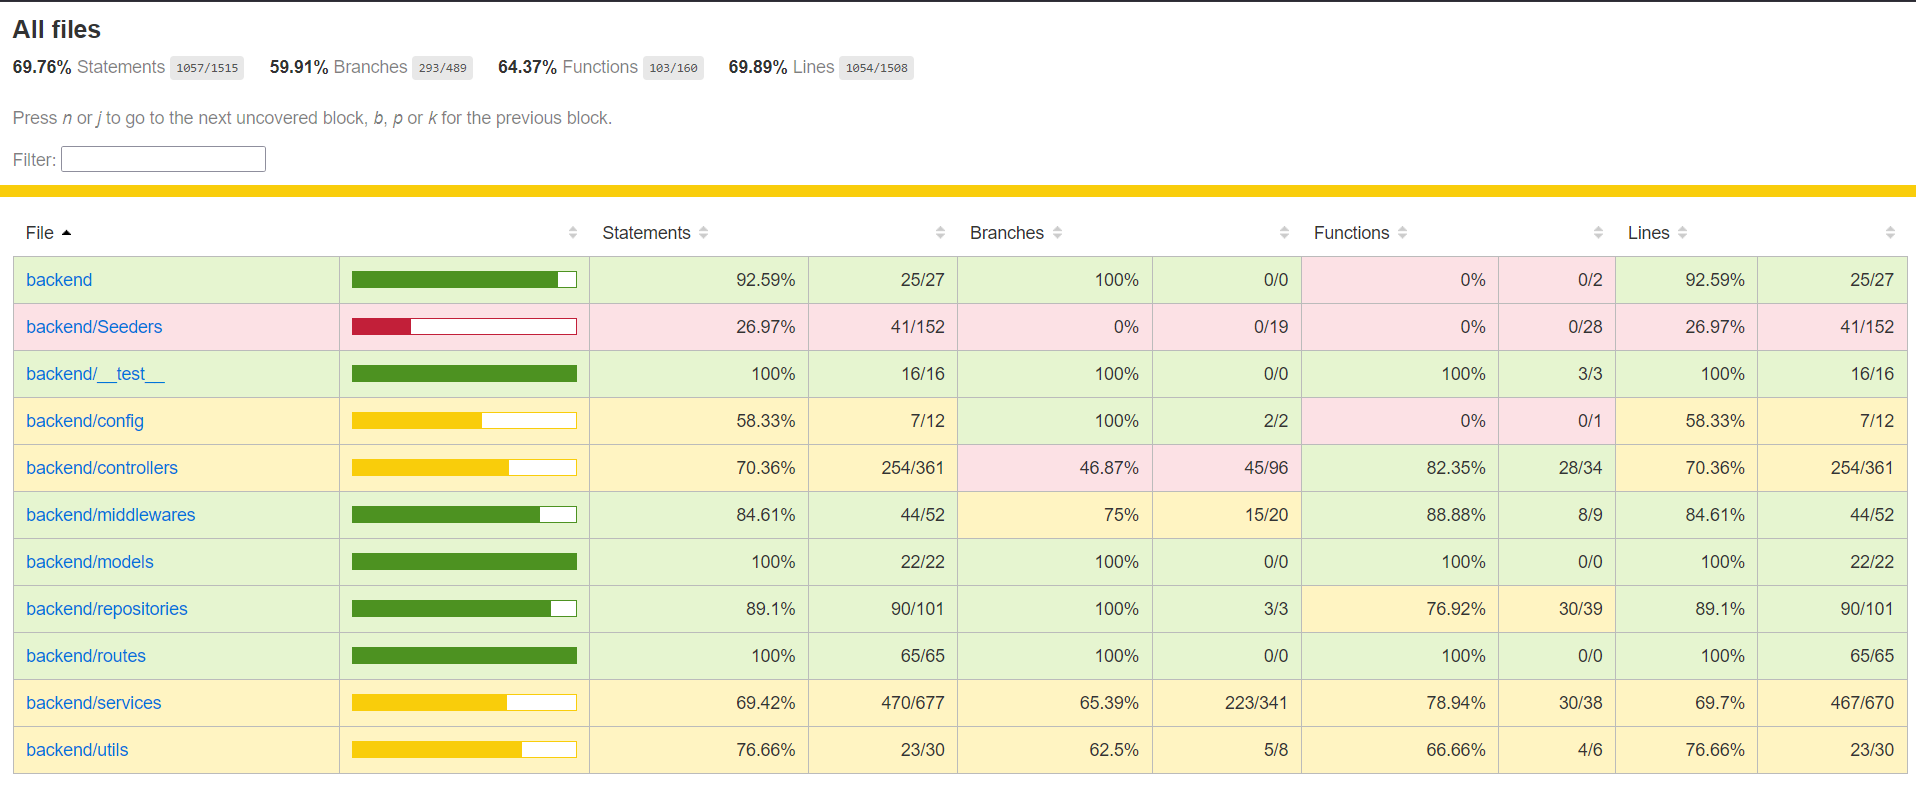
\includegraphics[clip=true,width=\textwidth]{img/cobertura_backend_logart.png}\\

    \footnotesize (f)
  \end{minipage}
  \caption{Informe de Cobertura de Pruebas del Backend (Jest).}\label{fig:coberturaBackend}
  \end{figure}

  La implementación de esta estrategia de pruebas ha sido fundamental para asegurar la calidad y estabilidad de LogArt durante su desarrollo.

\section{Distribución y Despliegue}
\label{sec:distribucionDespliegueCap4}

La capacidad de empaquetar la aplicación de forma consistente y desplegarla en diferentes entornos es crucial. LogArt utiliza Docker para la contenerización y GitHub Actions para automatizar la creación y publicación de imágenes, facilitando tanto el desarrollo local como una eventual puesta en producción.

\begin{itemize}
    \item \textbf{Empaquetado con Docker (\texttt{Dockerfile}):}
    \begin{itemize}
        \item La aplicación LogArt se empaqueta como una imagen Docker utilizando un \textbf{Dockerfile} multi-etapa, tal como se describió en la Sección \ref{sec:contenedores}.
        \item Este \texttt{Dockerfile} primero construye el frontend React en una etapa llamada (\textbf{frontend-build}, luego compila el backend Node.js en otra (\textbf{backend-build}), optimizando las dependencias y eliminando las de desarrollo.
        \item Finalmente, una etapa de producción basada en \texttt{node:20-alpine} copia los artefactos compilados del backend y el frontend (este último a una carpeta \texttt{/public} dentro del backend), resultando en una imagen final ligera y optimizada que contiene la aplicación completa lista para ejecutarse. La aplicación se configura para ejecutarse en el puerto 8443 en modo producción.
    \end{itemize}
    \vspace{0.3cm}
    \item \textbf{Orquestación Local con Docker Compose (\textbf{docker-compose.yml}):}
    \begin{itemize}
        \item Para el entorno de desarrollo local y pruebas, se utiliza el archivo detallado en la Sección \ref{ssec:arquitecturaDespliegue}: \textbf{\texttt{docker-compose.yml}} 
        \item Este archivo define y orquesta los dos servicios principales: \texttt{app} (que ejecuta la imagen Docker de LogArt) y \texttt{mongo} (que ejecuta la base de datos MongoDB).
        \item Configura las variables de entorno necesarias (cargadas desde un archivo \texttt{.env} para el servicio \texttt{app}), las redes para la comunicación entre contenedores, junto con los puertos expuestos.
        \item incluye \textit{healthchecks} para ambos servicios, asegurando un arranque ordenado y la correcta operatividad del sistema.
        \item Permite levantar todo el entorno con un simple comando (\texttt{docker-compose up}), lo que simplifica enormemente la configuración para cualquier desarrollador o para ejecutar la aplicación en un entorno de demostración. Las instrucciones detalladas para la ejecución se encuentran en el \texttt{README.md} del proyecto.
    \end{itemize}
    \vspace{0.3cm}
    \item \textbf{Distribución de Imágenes mediante CI/CD (GitHub Actions y DockerHub):}
    \begin{itemize}
        \item El proceso de construcción y distribución de la imagen Docker de LogArt está automatizado mediante el workflow de Entrega Continua en GitHub Actions, como se explicó en la Sección \ref{sec:cicd}.
        \item Cuando se publica una nueva \textit{release} en GitHub, este workflow se activa automáticamente, construye la imagen Docker de la aplicación utilizando el \texttt{Dockerfile} del proyecto.
        \item La imagen construida se etiqueta con múltiples tags (versión semántica, \texttt{latest} para releases estables, y hash del commit) y se publica en un registro público de contenedores, \textbf{DockerHub} (bajo el repositorio ``davidmorenoo/logartapp''.
        \item Esta automatización asegura que cada release estable de la aplicación esté disponible como una imagen Docker lista para ser utilizada, ya sea para despliegues manuales o mediante sistemas más avanzados.
        \item Tras la publicación de una nueva imagen, el archivo \texttt{docker-compose.yml} del proyecto (que está inicialmente configurado para usar una etiqueta específica, \texttt{latestManual}) puede ser actualizado manualmente para apuntar a la nueva versión de la imagen publicada en DockerHub si se desea utilizar la versión más reciente (última release) o apuntar a una versión anterior.
        \end{itemize}
        \vspace{0.3cm}
        \item \textbf{Consideraciones para un Futuro Despliegue en Producción (Conceptual):}
        \begin{itemize}
            \item Aunque este TFG se centra en el desarrollo y la demostración en un entorno local dockerizado, la arquitectura y el empaquetado con Docker facilitan un eventual despliegue en un entorno de producción.
            \item Se podrían utilizar plataformas de servicios en la nube que soporten contenedores Docker (ej. Amazon ECS, Google Kubernetes Engine, o plataformas PaaS como Heroku o Railway que permiten desplegar desde imágenes Docker).
            \item En un entorno de producción, se deberían utilizar certificados SSL válidos emitidos por una Autoridad de Certificación (CA) en lugar de los autofirmados, y la gestión de secretos (como claves de API, contraseñas de base de datos, etc) se realizaría mediante sistemas de gestión de secretos específicos de la plataforma de nube utilizada, o herramientas como HashiCorp Vault.
            \item La base de datos MongoDB podría desplegarse como un servicio gestionado (ej. MongoDB Atlas) para mayor escalabilidad y resiliencia.
        \end{itemize}
\end{itemize}

Este enfoque de distribución y despliegue basado en contenedores y CI/CD asegura la reproducibilidad, facilita la gestión de la aplicación y sienta las bases para una operativa futura eficiente.